\documentclass[a4paper,12pt, twoside]{scrreprt}
% Autor der Vorlage: Klaus Rheinberger, FH Vorarlberg
% 2017-02-20

%% Hilfe: z.B.
% empfohlener Einstieg: http://latex.tugraz.at/  
% https://de.wikibooks.org/wiki/LaTeX-Kompendium:_Schnellkurs:_Erste_Schritte
% https://de.wikibooks.org/wiki/LaTeX-Kompendium:_Schnellkurs
% https://de.wikibooks.org/wiki/LaTeX-Kompendium

%% Pakete:
% Der Befehl \usepackage[latin9]{inputenc} ermöglicht die direkte Angabe von Umlauten. Übrigens lässt sich so auch das Euro-Zeichen direkt eingeben. Auf Betriebssystemen, wie zum Beispiel allen neueren Linux-Distributionen, verwendet man statt \usepackage[latin9]{inputenc} besser \usepackage[utf8]{inputenc}, auf Applesystemen verwendet man \usepackage[macce]{inputenc} (oder das für ältere Modelle gültige \usepackage[applemac]{inputenc}).
\usepackage[utf8]{inputenc}
\usepackage[T1]{fontenc}    % Silbentrennung bei Sonderzeichen
\usepackage{graphicx}       % Bilder einbinden
\usepackage[ngerman]{babel} % Deutsche Sprachanpassungen
\usepackage{csquotes}       % When using babel or polyglossia with biblatex, loading csquotes is recommended to ensure that quoted texts are typeset according to the rules of your main language.
\usepackage{acronym}  % für optionales Abkürzungsverzeichnis
\usepackage{eurosym}  % z. B. \EUR{12345,68}
\usepackage[linktocpage=true]{hyperref} % Links z. B. \href{https://www.wikibooks.org}{Wikibooks home}
\usepackage{caption} % Abbildungslegenden
\captionsetup{format=hang, justification=raggedright}
%\usepackage[style=alphabetic,citestyle=alphabetic,backend=bibtex]{biblatex}   % Literaturverweise

%% own packages
\usepackage{longtable}
\usepackage{ragged2e}
\usepackage[german]{datetime2}
\usepackage{listings}
\usepackage[style=alphabetic,citestyle=alphabetic,backend=bibtex,block=ragged]{biblatex}
\addbibresource{bibresource.bib}

\usepackage{color}
%\usepackage[dvipsnames]{xcolor}
\usepackage[table, dvipsnames]{xcolor}
\usepackage{paralist}
\usepackage{svg}
\usepackage{enumitem}
\usepackage{listings}
\usepackage[section]{placeins}
%Zitate
%\usepackage[superscript]{cite}
%\usepackage[numbers,round]{natbib}
\usepackage{diagbox}
\usepackage{tcolorbox}
\usepackage[T1]{fontenc}
\usepackage[utf8]{inputenc}
\usepackage{newunicodechar}
\usepackage{siunitx}
\sisetup{locale = DE}

\usepackage{tikz}
\usetikzlibrary{trees, shapes, arrows}

\usepackage{tabularx}
\usepackage{makecell}
\renewcommand\theadfont{\bfseries\sffamily}
\usepackage{xspace}

%\usepackage{multirow}
%\usepackage{booktabs}


\hyphenchar\font=\string"7F
\hyphenation{Online-Programmier-verfahren Be-schleu-ni-gung}

%setup pdf
\hypersetup{
	pdfauthor={Helmut Rhomberg}
	pdfkeywords={Bachelorarbeit, FHV, Node.js, Programmieren, Software Engineer, BSc, Mobile Apps, Server}
	pdftitle={Node.js als Server-Plattform für mobile Apps}
}

\definecolor{bluekeywords}{rgb}{0.13,0.13,1}
\definecolor{greencomments}{rgb}{0,0.5,0}
\definecolor{redstrings}{rgb}{0.9,0,0}
\setcounter{secnumdepth}{4}
\setcounter{tocdepth}{4}   % Tiefe der Gliederung im Inhaltsverzeichnis

% http://latexcolor.com/
% https://en.wikibooks.org/wiki/LaTeX/Colors

\definecolor{lightgray}{rgb}{.9,.9,.9}
\definecolor{darkgray}{rgb}{.4,.4,.4}
\definecolor{purple}{rgb}{0.65, 0.12, 0.82}

\lstdefinelanguage{JavaScript}{
	keywords={break, case, catch, continue, debugger, default, delete, do, else, false, finally, for, function, if, in, instanceof, new, null, return, switch, this, throw, true, try, typeof, var, void, while, with},
	morecomment=[l]{//},
	morecomment=[s]{/*}{*/},
	morestring=[b]',
	morestring=[b]",
	ndkeywords={class, export, boolean, throw, implements, import, this},
	keywordstyle=\color{blue}\bfseries,
	ndkeywordstyle=\color{darkgray}\bfseries,
	identifierstyle=\color{black},
	commentstyle=\color{purple}\ttfamily,
	stringstyle=\color{red}\ttfamily,
	sensitive=true
}

% hypenations
\hyphenation{Kos-ten-er-spar-nis-sen}
\hyphenation{An-wen-dung}

%% Einstellungen:
\setcounter{secnumdepth}{4}
\setcounter{tocdepth}{4}   % Tiefe der Gliederung im In haltsverzeichnis

% own macros

\newcommand{\acronymContainer}[1]{
	\begin{flushleft}
		\begin{longtable}{p{0.2\textwidth} p{0.8\textwidth}}
		#1
		\end{longtable}
	\end{flushleft}
}

\newcommand{\acronymEntry}[2]{
	\textbf{#1} & #2
}

\newcommand{\acronymEntryNewline}[0]{
	\vspace*{0.631em} \\
}

\newcommand{\todayWithoutDay}{\DTMlangsetup[german]{showdayofmonth=false}\today\DTMlangsetup[german]{showdayofmonth=true}}

\newcommand{\quoteMark}[1]{%
	\glqq#1\grqq%
}

\newcommand{\setCSharpListing}{
	\lstset{language=[Sharp]C,
		extendedchars=\true,
		escapeinside=``,
		inputencoding={utf8},
		showspaces=false,
		showtabs=false,
		breaklines=true,
		showstringspaces=false,
		breakatwhitespace=true,
		escapeinside={(*@}{@*)},
		commentstyle=\color{greencomments},
		keywordstyle=\color{bluekeywords}\bfseries,
		stringstyle=\color{redstrings},
		basicstyle=\ttfamily,
		captionpos=t
	}
}

\newcommand{\setBashListing}{
	\lstset{language=bash,
		extendedchars=\true,
		escapeinside=``,
		inputencoding={utf8},
		basicstyle=\ttfamily,
		showstringspaces=false,
		commentstyle=\color{red},
		keywordstyle=\color{blue},
		captionpos=t
	}
}

\newcommand{\setJavaScriptListing}{
	\lstset{language=JavaScript,
		extendedchars=\true,  
		escapeinside=``,
		inputencoding={utf8},
		extendedchars=true,
		basicstyle=\footnotesize\ttfamily,
		showstringspaces=false,
		showspaces=false,
		numberstyle=\footnotesize,
		numbersep=9pt,
		tabsize=2,
		breaklines=true,
		showtabs=false,
		captionpos=t
	}
}

\newcommand\YAMLcolonstyle{\color{red}\mdseries}
\newcommand\YAMLkeystyle{\ttfamily\color{black}\bfseries}
\newcommand\YAMLvaluestyle{\color{blue}\mdseries}

\makeatletter

\newcommand\language@yaml{yaml}

\expandafter\expandafter\expandafter\lstdefinelanguage
\expandafter{\language@yaml}
{
  keywords={true,false,null,y,n},
  keywordstyle=\color{darkgray}\bfseries,
  basicstyle=\YAMLkeystyle,                                 % assuming a key comes first
  sensitive=false,
  comment=[l]{\#},
  morecomment=[s]{/*}{*/},
  commentstyle=\color{purple}\ttfamily,
  stringstyle=\YAMLvaluestyle\ttfamily,
  moredelim=[l][\color{orange}]{\&},
  moredelim=[l][\color{magenta}]{*},
  moredelim=**[il][\YAMLcolonstyle{:}\YAMLvaluestyle]{:},   % switch to value style at :
  morestring=[b]',
  morestring=[b]",
  literate =    {---}{{\ProcessThreeDashes}}3
                {>}{{\textcolor{red}\textgreater}}1     
                {|}{{\textcolor{red}\textbar}}1 
                {\ -\ }{{\mdseries\ -\ }}3,
                %{\ }{{\copyablespace}}1,
  columns=fullflexible,
  keepspaces=true,
  showstringspaces=false,
  showspaces=false
}

% switch to key style at EOL
\lst@AddToHook{EveryLine}{\ifx\lst@language\language@yaml\YAMLkeystyle\fi}
\makeatother

\newcommand\ProcessThreeDashes{\llap{\color{cyan}\mdseries-{-}-}}

\makeatletter
\def\lst@outputspace{{\ifx\lst@bkgcolor\empty\color{white}\else\lst@bkgcolor\fi\lst@visiblespace}}
\makeatother


\newcommand{\bracketText}[1]{%
    \textit{\scriptsize{#1}}%
}

\newenvironment{compactenumerate}{
\begin{enumerate}
  \setlength{\itemsep}{1pt}
  \setlength{\parskip}{0pt}
  \setlength{\parsep}{0pt}
}{\end{enumerate}}

\newenvironment{redbox}[1]{
    \begin{tcolorbox}[colback=Red!20!White,colframe=Red!85!White,title={#1}]
    }{\end{tcolorbox}
}

% gender some words with macros

\newcommand{\entwicklerSi}{Entwickler}
\newcommand{\entwicklerinSi}{Entwicklerin}
\newcommand{\entwicklerPl}{Entwickler}
\newcommand{\entwicklerinPl}{Entwicklerinnen}
%\newcommand{\EntwicklerSi}{\entwicklerSi{}/\entwicklerinSi{}}
\newcommand{\EntwicklerSi}{\entwicklerinSi{}}
%\newcommand{\EntwicklerPl}{\entwicklerPl{}/\entwicklerinPl{}}
\newcommand{\EntwicklerPl}{\entwicklerinPl{}}
%\newcommand{\demEntwickler}{dem \entwicklerSi{}/der \entwicklerinSi{}}
\newcommand{\demEntwickler}{der \entwicklerinSi{}}
%\newcommand{\denEntwickler}{den \entwicklerSi{}/die \entwicklerinSi{}}
\newcommand{\denEntwickler}{die \entwicklerinSi{}}
%\newcommand{\derEntwickler}{der \entwicklerSi{}/die \entwicklerinSi{}}
\newcommand{\derEntwickler}{der \entwicklerinSi{}}
\newcommand{\desEntwicklers}{des \entwicklerSi{}s}
\newcommand{\dieEntwickler}{die \entwicklerinPl{}}

% to avoid an issue
\newcommand{\dieEntwicklerin}{die \entwicklerinSi{}}

\newcommand{\mitarbeiterSi}{Mitarbeiter}
\newcommand{\mitarbeiterinSi}{Mitarbeiterin}
\newcommand{\mitarbeiterPl}{Angestellten}
\newcommand{\derMitarbeiterPl}{der \mitarbeiterPl{}}

%\newcommand{\benutzerSi}{Anwendende}
\newcommand{\benutzerSi}{User}
%\newcommand{\benutzerPl}{Anwendenden}
\newcommand{\benutzerPl}{User}
\newcommand{\derBenutzer}{der \benutzerSi{}}
\newcommand{\DerBenutzer}{Der \benutzerSi{}}
\newcommand{\einenBenutzer}{einen \benutzerSi}
\newcommand{\desBenutzers}{des \benutzerSi s}
\newcommand{\denBenutzer}{den \benutzerSi}
\newcommand{\demBenutzer}{dem \benutzerSi}
\newcommand{\DemBenutzer}{Dem \benutzerSi}

\newcommand{\ingenieurSi}{diplomierte technische Fachkraft}
\newcommand{\ingenieurPl}{diplomierten technischen Fachkräften}
\newcommand{\vondenIngenieuren}{von den \ingenieurPl{}}

\newcommand{\kundeSi}{Kunde}
\newcommand{\kundinSi}{Kundin}
\newcommand{\kundePl}{Kunden}
\newcommand{\kundinPl}{Kundinnen}
%\newcommand{\demKunden}{dem \kundeSi{}/der \kundinSi{}}
\newcommand{\demKunden}{der \kundinSi{}}
\newcommand{\dieKunden}{die \kundePl{}}
%\newcommand{\derKunden}{der \kundePl{}}
\newcommand{\derKunden}{der \kundinPl{}}


%% ERSETZEN VON ECKIGEN KLAMMERN:
% Ersetzen Sie den Text in den eckigen Klammern!

\begin{document}
\raggedbottom % http://www.weinelt.de/latex/raggedbottom.html

% evtl. Sperrvermerkseite
%\thispagestyle{empty}
%[Achtung: Verwenden Sie einen Sperrvermerk nur in sehr gut begründeten Fällen!] 

%\section*{Sperrvermerk}   % evtl. ersetzen durch \section*{Sperrvermerk}
%Auf Wunsch der Firma Creasoft AG ist die vorliegende Arbeit bis zum [DATUM] für die öffentliche Nutzung zu sperren. 

%Veröffentlichung, Vervielfältigung und Einsichtnahme sind ohne ausdrückliche Genehmigung der oben genannten Firma und der/dem %Verfasser/in nicht gestattet. Der Titel der Arbeit sowie das Kurzreferat/Abstract dürfen jedoch veröffentlicht werden.

%\vspace{3cm}

%\noindent Dornbirn, \todayWithoutDay \hfill Helmut Rhomberg

%\vspace{2cm}

%\hfill Firmenstempel\hspace{2cm}


% Titelblatt:
% \newpage\mbox{}\newpage
\cleardoublepage   % force output to a right page
\thispagestyle{empty}
\begin{titlepage}
  \begin{flushright}
  
\includegraphics[width=0.4\linewidth]{Logo-A3}
  \end{flushright}
  \begin{flushleft}
  \section*{Masterarbeit} %[Titel der Arbeit]
  \subsection*{\textcolor{red}{Teachen von Industrierobotern mittels Gestenerkennung (TODO: abändern?)}}
  \vspace{1cm}
  
  Masterarbeit\\
  zur Erlangung des akademischen Grades
  \vspace{0.5cm}
  
  \textbf{Master of Science in Engineering (MSc)} %[z. B. Master of Science in Engineering (MSc)]

  \vspace{1cm}
  Fachhochschule Vorarlberg\newline
  Informatik %[z. B. Energietechnik und Energiewirtschaft]

  \vspace{0.5cm}
  
  Betreut von\newline
  Dipl.-Ing. Robert Amann %[Name(n) der betreuenden Lehrperson(en)]
  
  \vspace{0.5cm}
  
  Vorgelegt von\newline
  Helmut Rhomberg\newline
  1810249003\newline\newline %[Name(n) der Verfasser/innen]\newline
  Dornbirn, \todayWithoutDay %[Monat Jahr]
  \end{flushleft}
\end{titlepage}

\newpage
\section*{Gender-Erklärung}
Der Verfasser der vorliegenden Arbeit bekennt sich zu einer geschlechtergerechten Sprachverwendung.\\

Um die Lesbarkeit zu gewährleisten und zugunsten der Textökonomie werden die verwendeten Personen bzw. Personengruppen fix männlich oder weiblich zugeordnet. Zum Beispiel werden immer die Entwicklerin, der Mitarbeiter, der Anwendende und die Kundin verwendet. Es wurde besonders darauf geachtet, stereotype Rollenbeschreibungen zu vermeiden.


% evtl. Widmung:
%\newpage
%\section*{Widmung}   % evtl. ersetzen durch \section*{Widmung}
%
%Nachfolgend möchte ich mich bei allen bedanken, welche mich während der Anfertigung %dieser Bachelorarbeit unterstützt haben.\\
%
%Ganz speziell bedanke ich mich bei:
%\begin{itemize}
%	\item Prof. Thomas Feilhauer für die Betreuung dieser Bachelorarbeit vonseiten der FH Vorarlberg und seine hilfreichen Verbesserungsvorschläge
%	\item Lukas Prutsch für dessen hilfreiche Ideen, um diese Arbeit zu verbessern
%	\item Paul Diem, welcher mich immer wieder dazu ermunterte an dieser Arbeit weiterzuschreiben
%	\item und allen anderen, ohne die diese Arbeit nicht so erfolgreich hätte sein können.
%\end{itemize}

% Kurzreferat:
\newpage
\section*{Kurzreferat}

\subsection*{\textcolor{red}{@TODO: Titel der Arbeit}}
\textcolor{red}{TODO}


% Abstract:
\newpage
\section*{Abstract}
\subsection*{\textcolor{red}{@TODO: Titel der Arbeit}}
The Teach Pendant has been used since its first appearance to teach industrial robots target poses so that they can then approach the target poses autonomously. The joystick or 3D mouse installed on the teach pendant for input makes it possible to realize very fine movements for the industrial robot. In addition, the teach pendant offers the possibility of teaching target poses to an industrial robot with little computing effort. This design decision was necessary, among other things, because the computational effort required to find paths independently would have been far too high at the time of the first teach pendants. In addition, it is not always possible to have the paths found independently by a software, since there is usually too little information available about the environment. Furthermore, inputs via natural user interfaces, such as gestures, were not yet sufficiently precise enough at that time.\\

Due to the rapid increase in computing capacity and the constant success in the research of artificial neural networks, gesture recognition systems have become the focus of research today. Gesture recognition systems promise intuitive and easy to learn operating concepts. The use of gestures also makes it possible to do without an additional device in the hands, thus enhancing the user experience. With heavy input devices, this can not only protect the arms but also the hands from signs of fatigue.\\

The goal of this thesis is therefore to create, test and analyze a gesture recognition system with and without ROS connection. The gesture information is provided by an Azure Kinect, but the depth camera and robot components are to remain interchangeable. The \quoteMark{WidowX 200} learning robot is used as the industrial robot for this purpose, as its small size means that it can be used easily and efficiently to test new functionalities. The gestures to be developed should above all provide high ergonomics and be secured against unintentional execution. Since the gestures have to be developed beforehand, it is therefore necessary to subject the gestures to practical tests in order to evaluate the ergonomics. The accuracy of gesture recognition also plays a major role in the tests to evaluate the ergonomics. The accuracy of the achieved target poses of the \quoteMark{WidowX 200} learning robot must be analyzed and latency tests must be performed to evaluate the gesture system as a whole.


% Inhaltsverzeichnis:
\cleardoublepage   % force output to a right page
\tableofcontents

\chapter{Einleitung}
Industrieroboter erfreuen sich heutzutage großer Beliebtheit bei Unternehmen um Produkte schnell und effizient herstellen zu können. Die Einsatzbereiche reichen hierbei von Laserschneiden über Schweißen und Fräsen bis hin zu Montageaufgaben, welche mitunter nur schwer von Personen durchgeführt werden können oder sogar lebensbedrohlich für Menschen sind. Zur Vermeidung von lebensbedrohlichen Situationen und zur Erleichterung von Vorgängen können Industrieroboter den Menschen hierbei effizient unterstützen und schwere Aufgaben erleichtern. Nichtsdestotrotz müssen von den Industrieroboterherstellern die geltenden Maschinenrichtlinien eingehalten werden um die Arbeit mit Menschen so gefahrlos wie nur möglich zu gestalten. Ein Beispiel hierfür ist das Erlernen bzw. Teachen von neuen Posen für einen Industrieroboter, sodass dieser seine Aufgaben im späteren Verlauf autonom durchführen kann. Hierzu muss sich die bedienende Person mitunter sehr nahe beim Industrieroboter befinden um Kollisionen mit Objekten frühzeitig erkennen und vermeiden zu können, aber auch um hohe Genauigkeiten für die zu erlernenden Zielposen zu erreichen. Zur Vermeidung von lebensbedrohlichen Situationen müssen die Industrieroboter beim Teachen deswegen unter anderem die Geschwindigkeit und Beschleunigung der Gelenke des Industrieroboters begrenzen.

\section{Umfeld}
Zum Teachen von Industrierobotern werden heutzutage vermehrt Teach Pendants eingesetzt, da durch deren Einsatz von Joystick und 3D-Maus als Eingabemethode sehr feine Bewegungen realisiert werden können. Zudem bietet das Teach Pendant durch das ergonomische Bedienen des \quoteMark{Enable device}-Schalters eine für Menschen sichere Möglichkeit einen Industrieroboter sicher zu bedienen. Bei zu starker oder zu schwacher Betätigung des \quoteMark{Enable device}-Schalters wird vom Teach Pendant eine Gefahrensituation angenommen und der Industrieroboter zum Stillstand gebracht um die bedienende Person vor lebensbedrohlichen Situationen zu schützen. Im Großen und Ganzen kann gesagt werden, dass ein Teach Pendant ein Multifunktionsgerät zur Programmierung von Industrierobotern darstellt und ohne großen Rechenaufwand und entsprechend komplizierten Algorithmen zum selbstständigen Finden der Wege auskommt. Diese Designentscheidung war unter anderem notwendig, da der Rechenaufwand zum selbständigen Finden von Wegen zu der Zeit der ersten Teach Pendants viel zu hoch gewesen wäre. Zudem ist es nicht immer möglich die Wege selbstständig von einer Software finden zu lassen, da zumeist zuwenige Informationen über die Umgebung bereitstehen. Daher musste eine alternative Möglichkeit entwickelt werden um Industrierobotern Posen beibringen zu können, welche anschließend autonom abgefahrt werden können. Die Möglichkeit dem Industrieroboter Posen mittels Teach Pendant zu erlernen hat sich aufgrund des Rechenaufwands daher bis heute als sehr hilfreich erwiesen. Aus diesem Grund haben sich Teach Pendants zum De-facto-Standard zur Programmierung von Industrierobotern entwickelt. Die Funktionalität der Teach Pendants wurde zudem um Hilfsfunktionen, wie z.B. Bewegungsmodi und Beschleunigungsanpassungen, und Hardwarefunktionalitäten, wie z.B. einen Touchpad, erweitert, um die Bedienung des Teach Pendants und so auch des Industrieroboters für die bedienende Person noch intutitiver zu gestalten.

\section{Problemstellung}
Obwohl Teach Pendants sehr weit verbreitet sind und sich über die Jahre als sehr hilfreich beim Teachen von Industrierobotern erwiesen haben, wird dennoch unter anderem durch den rasanten Anstieg der Rechenkapazität an neuen Eingabemethoden für Industrieroboter geforscht. Der am zukunftsweisendste Ansatz liegt in der Verwendung von NUI um der bedienenden Person die Bedienung des Industrieroboters mittels des eigenen Körpers so intutitiv wie nur möglich zu gestalten. Eine Möglichkeit eine natürliche Benutzterschnittstelle zu entwickeln besteht in der Verwendung von Gesten. Gesten sind intutitiv zu erlernen und einfach anzuwenden, wodurch die Verwendung eines zusätzlichen Geräts, wie z.B. eines Teach Pendants, entfällt. Bei schweren Eingabegeräten, welche in der Hand gehalten werden, ist dies besonders spürbar, da ein längeres Bedienen des Geräts zu Ermüdungserscheinungen in den Händen und Armen führen kann. In der Gestenerkennung wird aus diesem Grund eine einfache und intutitive Bedienungsmöglichkeit gesehen, welche eine ergonomischere Bedienung als mit einem herkömmlichen Teach Pendant ermöglichen kann. Die Sicherheitsaspekte dürfen dabei jedoch aber auch nicht vernachlässigt werden, da die Maschinenrichtlinien genauestens spezifizieren wie die zu bedienende Maschine mit Menschen interagieren muss um lebensbedrohliche Situationen zu vermeiden. Unter anderem muss hierfür die Geschwindigkeit und die Beschleunigung des Industrieroboters gedrosselt werden um es der bedienenden Person zu ermöglichen unbeabsichtigten Bewegungen des Industrieroboters zeitgerecht ausweichen zu können.

\section{Zielsetzung} \label{sec:zielsetzung} %Motivation
In dieser Arbeit stellt daher das Erstellen, Testen und Analysieren einer Gestenerkennung, welche die Tiefeninformationen von einer Tiefenkamera erhält, im Vordergrund. Hierbei sollen ergonomische Gesten entwickelt werden, welche nur schwer unbeabsichtigt durchgeführt werden können, die Genauigkeit der Gestenerkennung und der Zielposen analysiert und Latenztests durchgeführt werden. Zur genauen Umsetzung soll eine Azure Kinect als Tiefenkamera eingesetzt und der \quoteMark{WidowX 200}-Lernroboter zur Umsetzung und Überprüfung der Gestenerkkenung verwendet werden. Die zu erstellende Gestenerkennung soll jedoch nicht nur auf die Azure Kinect und den \quoteMark{WidowX 200}-Lernroboter beschränkt sein. Hierfür sollen deshalb Schnittstellen geschaffen werden, welche das einfache Austauschen der Tiefenkamera- und Roboter-Komponente ermöglichen sollen. Aus diesem Grund soll zudem ermittelt werden ob eine Anbindung über ROS hinsichtlich der Latenzen eine ernst zu nehmende Alternative zu einer direkten Kommunikation mit einem Industrieroboter darstellt. Daher soll eine konkrete Kommunikation über ROS und eine direkte Kommunikation mit dem \quoteMark{WidowX 200}-Lernroboter implementiert werden. Zu guter Letzt sollen die beiden Implementierungen auf Grundlage von Latenztests miteinander verglichen werden. Im Anschluss kann ein Fazit gezogen werden ob ROS den niedrigen Latenzenansprüchen von Industrierobotern gerecht werden kann. Alle in dieser Arbeit erstellten Dateien können zudem auf der beigefügten DVD oder im Github-Repository unter \href{https://github.com/TeachIndustrialRobots/Teach-Industrial-Robots}{https://github.com/TeachIndustrialRobots/Teach-Industrial-Robots} öffentlich eingesehen werden. Der Einfachkeitshalber wird die DVD oder das Github-Repository in dieser Arbeit als \quoteMark{Begleitmedium} bezeichnet.


\chapter{Stand der Technik} % Ausgangslage, Anforderungsanalyse
%Methodenwahl % Begründung der Auswahl

Industrieroboter können eine Vielzahl von verschiedenen Aufgabengebieten übernehmen. Die Aufgabengebiete reichen hierbei von Bedinungs- über Bearbeitungs- bis hin zu Montageabläufen \cite{industrieroboter_2020}. Die Schwierigkeit besteht hierbei zunächst die Anforderungen an den erforderlichen Industrieroboter zu definieren und wenn möglich einzugrenzen. Da die Kommunikation mit und ohne ROS getestet werden soll ist es von Vorteil einen Industrieroboter mit einer bereits vorhandenen ROS-Unterstützung zu verwenden. Zudem ist es erforderlich den Industrieroboter über eine direkte Schnittstelle ansprechen zu können um die gewünschten Abläufe, welche geteacht werden sollen, mit einer direkten Kommunikation ohne Netzwerklatenzen testen und einen Vergleich auf Grund des Zeitverhaltens anstellen zu können. Die Interoperabilität mit Simulationsumgebungen ist auch abzuwägen, da die Tests mithilfe einer Simulationsumgebung ohne Sicherheitsbedenken für die bedienende Person durchgeführt und zudem für Regressionstests der Gestenerkennungssoftware praktikabel ohne einen realen Roboter durchgeführt werden können. Im weiteren Verlauf muss zudem die Entscheidung für einen Tiefensensor durchgeführt werden um eine Gestenerkennung, welche zur Steuerung des Inustrieroboters eingesetzt werden soll, realiseren zu können. Bei der Gestenerkennung steht vor allem die Ergonomie und die Sicherheit der bedienenden Person im Vordergrund. Hierbei muss unter anderem beachtet werden, dass zufällige Gesten nicht als Aktion gewertet werden, da dies ansonsten die Sicherheit der bedienenden Person negativ beinflussen kann. Bei der Programmiersprache und Programmierumgebung ist dabei darauf zu achten, dass diese zu ROS kompatibel ist, da ansonsten erheblicher Mehraufwand bei der Umsetzung entstehen würde.

\section{Industrieroboter}
Ein Industrieroboter ist ein universell einsetzbarer Bewegungsautomat, welcher im industriellen Einsatzgebiet eingesetzt wird. Zu erwähnen ist, dass Industrieroboter zumeist auf ein bestimmtes Problem zugeschnitten sind. Aus diesem Grund werden diese je nach der Positionsgenauigkeit, Tragfähigkeit, Arbeitsbereich, Arbeitsgeschwindigkeit und maximaler Reichweite unterschieden. Die maximale Reichweite ist bei ortsfesten Industrierobotern durch die Armlänge und die Freiheitsgrade begrenzt. Im Gegensatz zu ortsfesten Industrierobotern können bewegliche Industrieroboter sich zusätzlich in der Umgebung bewegen und werden daher durch die Bewegungsvorrichtung begrenzt \cite{industrieroboter_2020}.

\begin{figure}[htb]
	\centering
	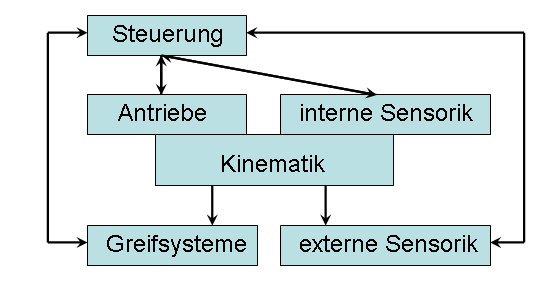
\includegraphics[width=0.6\textwidth]{images/stand_der_technik/Struktur_IR}
	\caption[Struktur eines Industrieroboters]{Struktur eines Industrieroboters \\Quelle: \cite{industrieroboter_2020}}
	\label{fig:struktur_eines_industrieroboters}
\end{figure}
\FloatBarrier

Wie in Abbildung \ref{fig:struktur_eines_industrieroboters} zu sehen ist, besteht ein Industrieroboter grundlegend aus einem Roboterarm, welcher auch Manipulator genannt wird, einer Steuerungseinheit, welche für die Überwachungung und Übersetzung der Aktionen auf den spezifischen Industrieroboter zuständig ist und einem Endeffektor, welcher über ein Greifsystem befestigt wird. Über den Manipulator, welcher Gelenke und Antriebe aufweist, wird die Kinematik realisiert, welche es ermöglicht den Manipulator im 3D-Raum zu bewegen. Um jeden Punkt im 3D-Raum ansteuern zu können sind mindestens 3 DOF erforderlich, welche über Gelenke realisiert werden. Um jeden Punkt im Raum mit jeder beliebigen Orientierung ansteuern zu können benötigt es jedoch 6 DOF, wobei 3 Gelenke für translatorische und weitere 3 Gelenke für rotatorische Bewegungsabläufe zuständig sind. Der Endeffektor kann auf verschiedene Arten realisiert werden. Zumeist ist es jedoch ein Werkzeug, welches z.B. für Schweiß-, Bohr-, Beschichtungs-, Klebe-, Montage- oder Schneidearbeiten eingesetzt werden kann. Da der Endeffektor austauschbar ist, besteht jedoch aber auch die Möglichkeit einen Greifer oder einen anderen spezifisch für eine Aufgabe konzipierten Endeffektor zu montieren und zu verwenden. Damit die Steuerungseinheit die Gelenkpositionen und Antriebsgeschwindigkeiten ermitteln kann sind zudem Messsysteme erforderlich, welche als interne Sensoren bezeichnet werden. Als optionale Komponente können zudem externe Sensoren beim Industrieroboter verbaut sein, welche unter anderem zur Ermittlung von Objektpositionen im 3D-Raum und deren Größen verwendet werden können. Je nach Arbeitsumfeld kann es auch erforderlich sein, dass ein System zum Wechseln des Endeffektors eingesetzt wird um mehrere Arbeitsschritte mit einem einzigen Industrieroboter durchführen zu können \cite{hagele_aufbau_2006}.

\subsection{Bauformen}
Industrieroboter können entweder zur seriellen oder parallelen Kinematik zugeordnet werden. Der Unterschied besteht darin, dass die Achsen bei der seriellen Kinematik seriell angeordnet sind, wohingegen bei der paralleln Kinematik die Achsen parallel angeordnet werden.

\begin{figure}[htb]
	\centering
	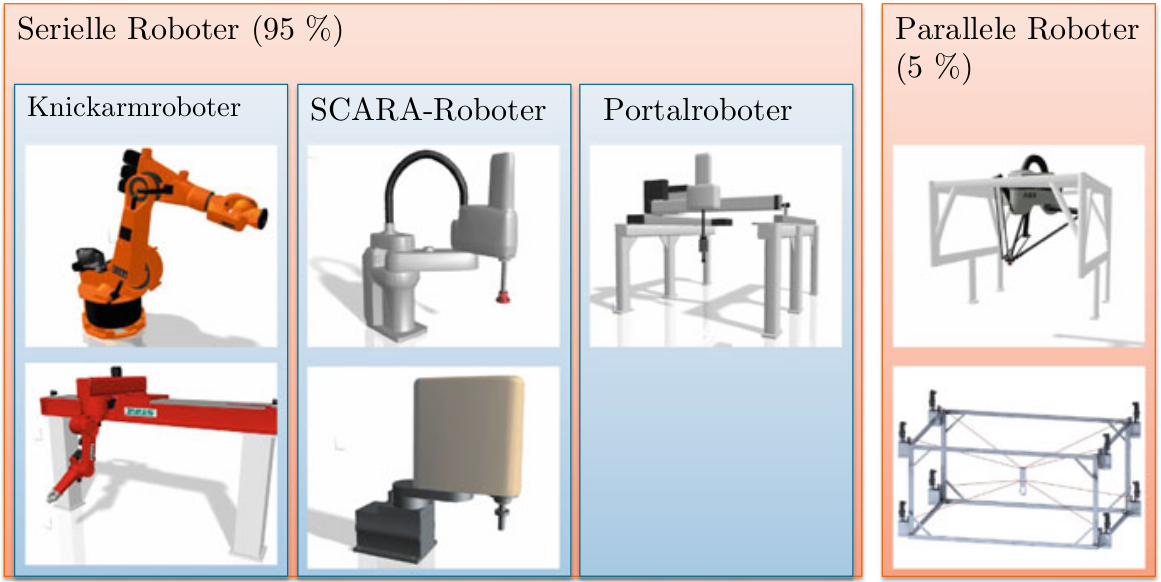
\includegraphics[width=0.9\textwidth]{images/stand_der_technik/bauformen_industrieroboter}
	\caption[Bauformen von Industrierobotern]{Bauformen von Industrierobotern \\Quelle: \cite[18]{pott_industrielle_2019}}
	\label{fig:bauformen_industrieroboter}
\end{figure}
\FloatBarrier

Mit 95\% Anteil haben sich Industrieroboter mt serieller Kinematik aufgrund ihrer Bauweise und den bei Knickarmrobotern sehr großen Bewegungsfreiheit durchgesetzt, wie aus der Abbildung \ref{fig:bauformen_industrieroboter} zu entnehmen ist. Nur ein geringer Teil von 5\% der Industrieroboter besitzen eine parallele Kinematik, zu denen unter anderem der Delta- und Seil-Roboter zählen. In der Abbildung \ref{fig:bauformen_industrieroboter} ist der Delta-Roboter im Bereich der parallen Roboter oben und der Seilroboter im unteren Bereich zu sehen. Die parallele Kinematik zeichnet sich dabei durch mindestens eine geschlossene kinematische Kette aus. Zu den seriellen Industrierobotern zählen unter anderem Knick-, SCARA- und Portal-Roboter und alle anderen Roboter, welche eine offene kinematische Kette aufweisen. Industieroboter mit serieller Kinematik zählen zu den am weitest verbreitesten Industrierobotern. Im Gegensatz zu den seriellen Industrierobotern bieten parallele Industrieroboter durch die direkte Verbindung zum Greifsystem den Vorteil, dass die nachfolgenden Glieder und deren Massen nicht wie beim seriellen Industrieroboter die Dynamik des Systems beeinflussen können. Dies führt dazu, dass eine sehr hohe Genauigkeit und eine sehr hohe Steifigkeit garantiert werden kann. Zudem sind durch die parallele Kinematik hochpräzise Ansteuerungsmanöver mit sehr hoher Geschwindigkeit durchführbar. Der Nachteil besteht jedoch darin, dass parallele Industrieroboter ortsfest sind. Die parallele Kinematik zählt daher eher zur Ausnahme und wird aus diesem Grund vermehrt für Pick-and-Place-Aufgaben oder Sondermaschinen eingesetzt, wo Geschwindigkeit, eine hohe Präzision und hohe Dynamik erforderlich sind \cite[17\psqq]{pott_industrielle_2019}.\\

Der Knickarmroboter, welcher zu den seriellen Industrierobotern zählt und zumeist 6 DOF aufweist, bietet den Vorteil, dass dieser für weitere Bewegungsfreiheit auf eine zusätzliche Linearachse montiert werden kann. Dadurch ist es unter anderem Möglich verschiedene Arbeitspositionen eines großen Objekts ansteuern zu können. Da der Knickarmroboter eine armartige Form aufweist, ist dieser zumeist für schwer erreichbare Stellen geeignet. Aufgrund der offenen kinematischen Kette und der Möglichkeit einer sehr großen Nutzlast leidet jedoch die Absolutgenauigkeit darunter. Typischwerweise werden Knickarmroboter für Schweiß-, Handhabungs- und Klebearbeiten eingesetzt. Eine weitere Möglichkeit um serielle Industrieroboter zu realisieren stellen die SCARA-Roboter dar. Diese weisen im Gegensatz zu den Knickarmrobotern weniger Freiheitsgrade auf. Typischwerweise werden zumeist 3 oder 4 DOF verbaut, wodurch die Bewegungsfreiheit eingeschänkt wird. Zudem sind aufgrund der Bauform nur geringere Arbeitslasten und kleinere Arbeitsbereiche nutzbar. Dies zeigt sich auch im Aufgabengebiet, welches großteils aus der Montage und \quoteMark{Pick-and-Place}-Aufgaben besteht. Portale, welche auch zu den seriellen Industrierobotern zählen, können sehr hohe Nutzlasten und große Bewegungen durchführen. Sie sind nach den Knickarmrobotern die zweithäufigste Bauform. Zu den Aufgabengebieten zählen Pick-and-Place, Maschinenbestückungen und Kommisionsarbeiten \cite[17\psqq]{pott_industrielle_2019}.

\subsection{Positions- und Bahngenauigkeit}
Um Genauigkeitsmessungen an einem Industrieroboter durchzuführen ist es erforderlich die spezifischen Genauigkeiten eines Industrieroboters zu kennen und diese in einen Zusammenhang bringen zu können. Bei Industrierobotern ist die Genauigkeit in sehr vielen Aufgabenbereichen, wie z.B. Laserschneiden oder Schweißen, sehr entscheident. Eine hohe Genauigkeit spart Kosten und Zeit ein, da eine teure und zeitintensive Nachbearbeitung entfällt. Aus diesem Grund ist es entscheident, dass der Industieroboter für spezielle Aufgabenbereiche eine hohe Positions- und Bahngenauigkeit aufweist. Um die Positions- und Bahngenauigkeit von Industrierobotern beurteilen zu können verwendet man die Absolut- und Wiederholgenauigkeit. Beide Kennwerte beschreiben die Qualität der Übereinstimmung der Realität und des Modells und sind in der ISO 9283, welche die Robotergenauigkeit beinhaltet und beschreibt, standardisiert \cite[28\psqq]{pott_industrielle_2019}.

\begin{figure}[htb]
	\centering
	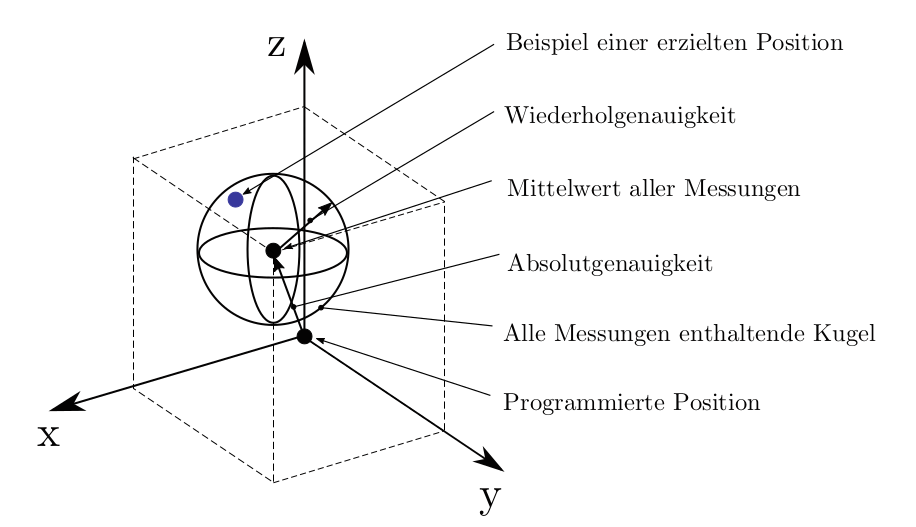
\includegraphics[width=0.686\textwidth]{images/stand_der_technik/absolutgenauigkeit_und_wiederholgenauigkeit}
	\caption[Absolut- und Wiederholgenauigkeit]{Absolut- und Wiederholgenauigkeit \\Quelle: \cite[29]{pott_industrielle_2019}}
	\label{fig:absolutgenauigkeit_und_wiederholgenauigkeit}
\end{figure}
\FloatBarrier

In der Abbildung \ref{fig:absolutgenauigkeit_und_wiederholgenauigkeit} ist der Zusammenhang zwischen der Absolut- und Wiederholgenauigkeit zu erkennen. Die Wiederholgenauigkeit wird ermittelt indem der Industrieroboter über mehrere Zyklen hinweg immer wieder die gleiche Pose aus einer spezifischen Richtung anfährt. Am Ende werden die dabei entstandenen Abweichungen gemittelt um die Wiederholgenauigkeit zu erhalten. Hierbei beeinflussen systematische Gegebenheiten, wie z.B. termische Ausdehnung durch Umgebungstemperatur, sowie aber auch durch die Motorwärme, Justagefehler der Achsen, Fertigungstoleranzen oder sogar Kollisionen die Genauigkeit des Gesamtsystems um die Zielpose exakt ansteuern zu können. Aus diesen Gründen ist es empfehlenswert den Industrieroboter jährlich auf die Genauigkeit zu prüfen und gegebenenfalls zu justieren. Im Gegensatz zur Wiederholgenauigkeit beschreibt die Absolutgenauigkeit wie genau der Industrieroboter eine theoretisch programmierte Zielpose, welche z.B. mittels CAD-Software erlernt wurde, im Bezug zum Roboterkoordinatensystem im Durchschnitt aus einer beliebigen Richtung ansteuern kann. Standardmäßig beträgt die Wiederholgenauigkeit bei Industrierobotern \num{0,1} mm wohingegen die Absolutgenauigkeit standardmäßig eine maximale Abweichung von 1 mm aufweist \cite[28\psqq]{pott_industrielle_2019}.

\begin{figure}[htb]
	\centering
	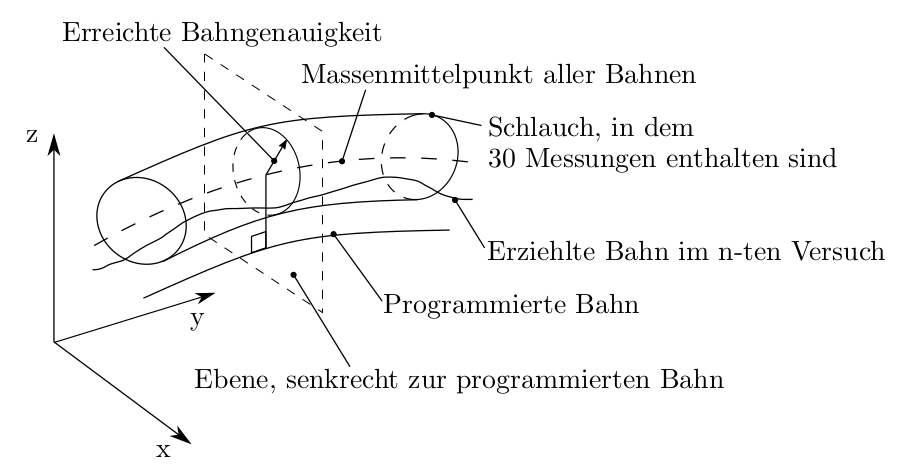
\includegraphics[width=0.735\textwidth]{images/stand_der_technik/bahngenauigkeit}
	\caption[Bahngenauigkeit]{Bahngenauigkeit \\Quelle: \cite[30]{pott_industrielle_2019}}
	\label{fig:bahngenauigkeit}
\end{figure}
\FloatBarrier

Bei einer großen Abweichung der Absolutgenauigkeit führt dies jedoch zu einem schlechteren erreichen der Zielpose und dadurch auch zu einem schlechteren Bahnverhalten, wie in Abbildung \ref{fig:bahngenauigkeit} durch die erzielte Bahn im n-ten Versuch ersichtlich ist. Die erzielte Bahn weist deutliche Schwingungen auf und weicht daher erkennbar von der zuvor programmierten Bahn ab. Aus diesem Grund bieten viele Hersteller gegen einen Aufpreis absolutvermessene Industrieroboter an um diesen Genauigkeitsfehler zu kompensieren \cite[29\psq]{pott_industrielle_2019}. Wenn eine sehr hohe Wiederholgenauigkeit gewünscht ist kann auch mit Spezialrobotern eine Wiederholgenauigkeit von bis zu 1 \si{\micro}m erreicht werden \cite{genauigkeit_nodate}.

\begin{figure}[htb]
	\centering
	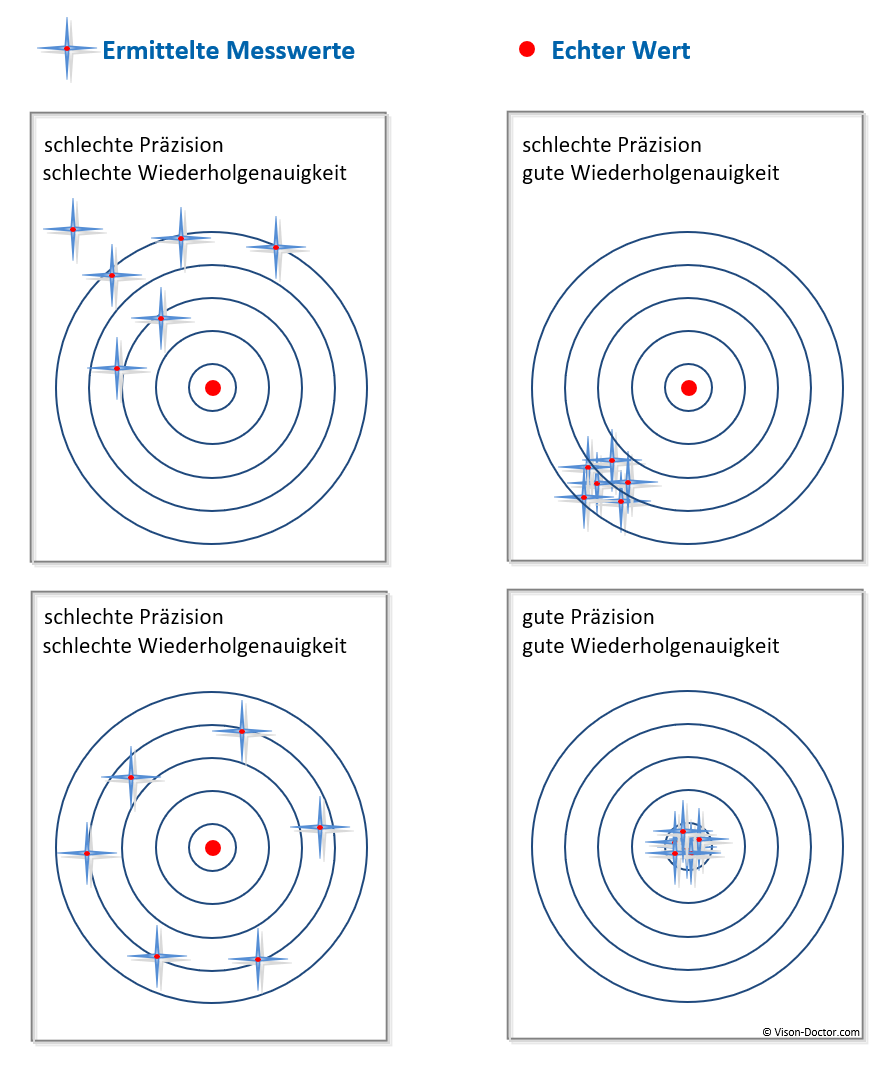
\includegraphics[width=0.57\textwidth]{images/stand_der_technik/wiederholgenauigkeit}
	\caption[Wiederholgenauigkeit]{Wiederholgenauigkeit \\Quelle: \cite{prazision_nodate}}
	\label{fig:wiederholgenauigkeit}
\end{figure}
\FloatBarrier

Wie in Abbildung \ref{fig:wiederholgenauigkeit} zu sehen ist, kann daraus geschlossen werden, dass keine hohe Präzision durch eine schlechte Wiederholgenauigkeit möglich ist. Aus diesem Grund kann auch gesagt werden, dass die Wiederholgenauigkeit entscheidenter als die Absolutgenauigkeit zum erreichen der Zielposition ist, da umgekehrt nicht gesagt werden kann, dass eine hohe Präzision durch eine gute Wiederholgenauigkeit erreicht werden kann \cite{genauigkeit_nodate}.

\section{Teachen von Industrierobotern}
Teachen, welches auch als Teach-In bezeichnet wird, ist eine von mehreren möglichen Varianten einem Industrieroboter gewünschte Posen beizubringen damit dieser seine Arbeitsaufgabe autonom durchführen kann.

\subsection{Offline- und Online-Programmierverfahren}
Unterschieden wird bei den Lernmethoden zwischen Offline- und Online-Programmierverfahren. Die am weitest verbreitesten Offline-Methoden sind die textuelle Programmierung und das Erlernen mit einer CAD-Software. Bei der textuellen Programmierung ist es notwendig über ausreichend Programmierkenntnisse in der Programmiersprache des Industrieroboter-Herstellers oder einer kompatiblen Programmiersprache zu verfügen, wohingegen bei einer CAD-Software einem virtuellen Industrieroboter in einer virtuellen Umgebung die zu erlernenden Posen beigebracht werden können. Beide Methoden benötigen im Vergleich zum Teachen sehr viel mehr Vorwissen und sind daher nur nach erheblichem Lernaufwand nutzbar. Das Teachen zählt neben der Playback-Methode, welche ein direktes Führen des Roboterarms ermöglicht, zu den Online-Programmierverfahren. Beim Teachen kommt eine Steuerkonsole zum Einsatz mit deren Hilfe es möglich ist dem Industrieroboter Posen beizubringen. Zuerst wird eine Pose mit mehreren aufeinander folgenden Steuerungsbefehlen angefahren. Anschließend, wenn eine gewünschte Pose erreicht wurde, kann diese einzelne Pose per Steuerungsbefehl in der Steuerungseinheit gespeichert werden. Das Anfahren und Speichern der Posen wird solange wiederholt bis die gesamte Arbeitsaufgabe dem Industrieroboter beigebracht wurde. Wenn notwendig, können im Nachhinein die gespeicherten Posen korrigiert werden um eine höhere Genauigkeit zu erzielen oder um Fehler zu korrigieren. Im Gegensatz zum Teachen wird beim Playback-Verfahren genau die Bewegung gespeichert, welche durch das direkte Führen des Roboterarms entsteht, und beim Ausführen der Arbeitsaufgabe auf die gleiche Weise wiederholt \cite{industrieroboter_2020}. Beim Teachen hingegen kann zwischen den Zielpunkten die Geschwindigkeit, Beschleunigung und sogar die Art des Pfades eingestellt werden. Bei der Art des Pfades kann frei zwischen Point-to-Point und Continuous Path gewählt werden. Point-to-Point erzwingt den für den Industrieroboter geometrisch günstigsten Pfad zwischen den Punkten zu wählen, welcher normalerweise keine gerade lineare Bahnbewegung darstellt und daher zu einem unbekannten Pfad führt. Bei Continuous Path wird hingegen von einem Punkt direkt zum nächsten Punkt entlang eines vordefinierten Pfades gefahren, welcher z.B. eine gerade lineare oder eine durch einen Hilfspunkt erzeugte kreisförmige Bahnbewegung sein kann. Durch diese Einstellungsmöglichkeiten ist es beim Teachen möglich noch höhere Genauigkeiten als bei der Playback-Methode zu erzielen. Im Gegenzug steigt durch die höhere Genauigkeit, aber auch der Programmieraufwand, da für eine hohe Genauigkeit viele Zwischenpunkte beigebracht werden müssen \cite{teach-technik_2020}.\\

Für alle Programmierverfahren, ob Offline- oder Online-Programmierverfahren, welche zur Programmierung von Industrierobotern eingesetzt werden können, kann gesagt werden, dass jedes Verfahren einen gewissen Lernaufwand bei der Einarbeitung benötigt. Der Lernaufwand um ein Programmierverfahren zu erlernen sinkt jedoch erheblich für untrainierte Personen, wenn eine visuelle Lernmethode eingesetzt wird. In Zukunft besteht daher ein sehr großes Potenzial zur Erforschung und Verbesserung von Gesten, Sprach und visuellen Systemen, da diese Systeme eine für den Menschen vertrauliche Interaktionsmöglichkeit bieten \cite{biggs_survey_nodate}.\clearpage

\subsection{Teach Pendant}
\begin{figure}[htb]
	\centering
	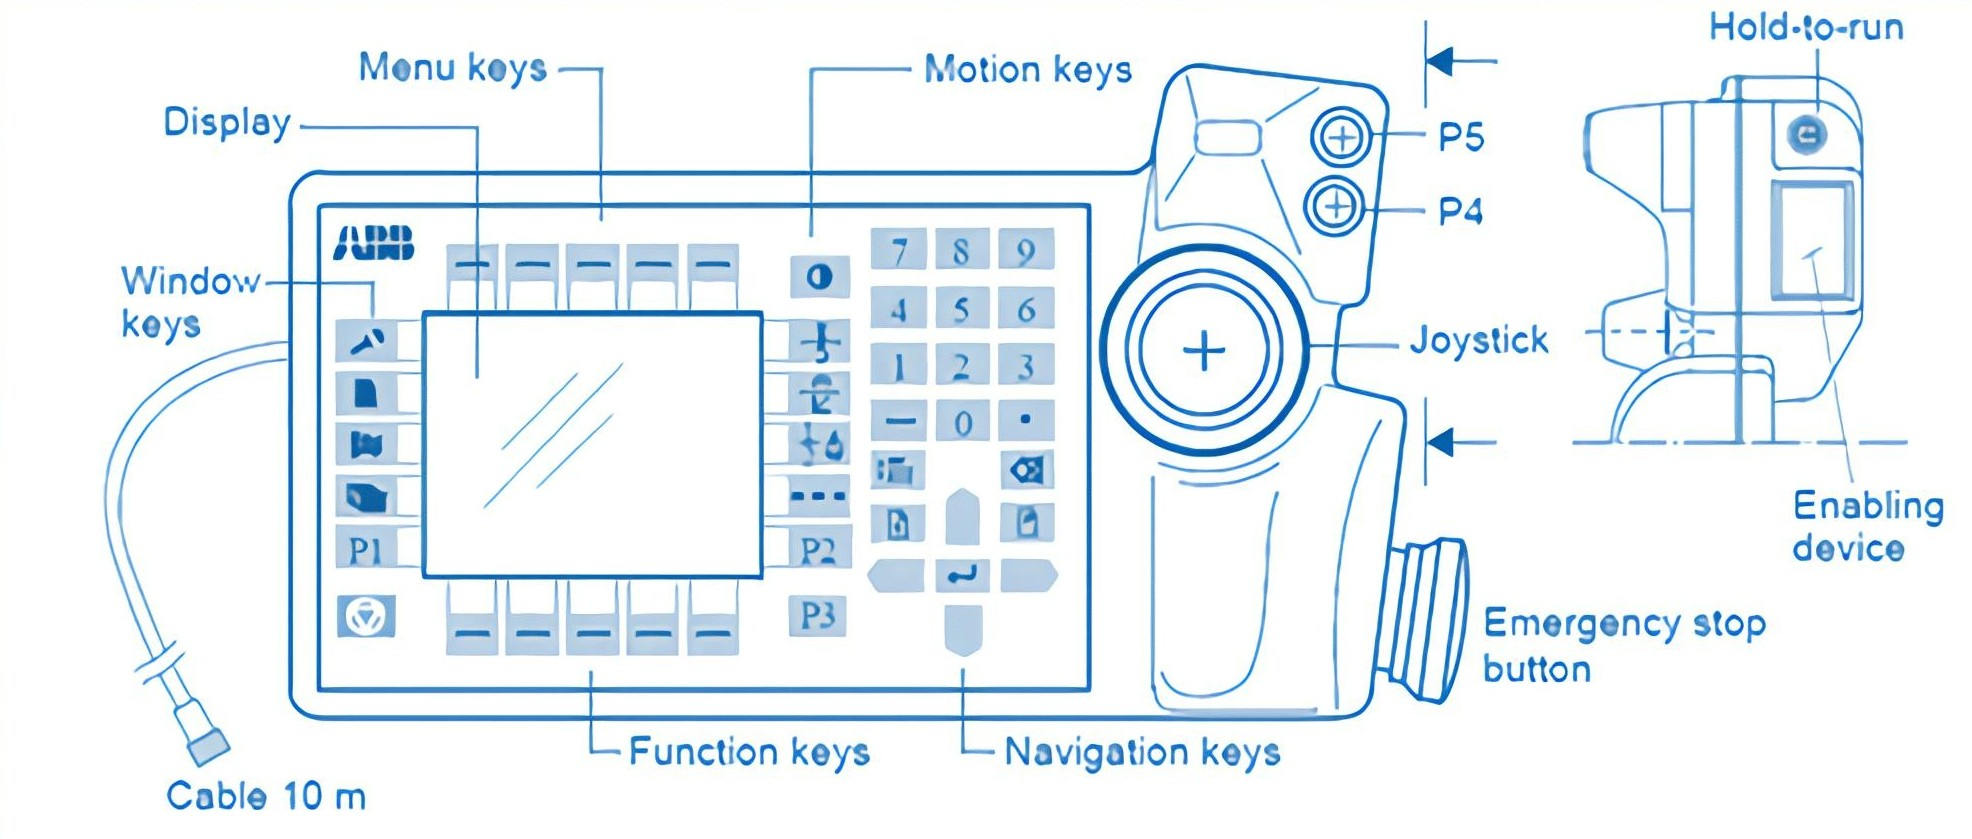
\includegraphics[width=0.715\textwidth]{images/stand_der_technik/teach_pendant}
	\caption[Teach Pendant im Querformat von ABB]{Teach Pendant im Querformat von ABB \\Quelle: \cite{programengif_nodate}}
	\label{fig:teach_pendant}
\end{figure}
\FloatBarrier

Zur Programmierung mit dem Teach-In-Verfahren werden Teach Pendants, wie in Abbildung \ref{fig:teach_pendant} zu sehen, eingesetzt, welche im Gegensatz zu früheren Modellen je nach Hoch- oder Querformat im oberen oder im linken Bereich des Teach Pendants über ein Display mit oder ohne Touch-Funktionalität verfügen \cite{nof_handbook_1999}. Unterschieden wird bei den herstellerspezifischen Teach Pendants zwischen dem Hoch- und Querformat. Beim Hochformat wird das Teachpendant mit beiden Händen gehalten und mithilfe der Daumen werden die Knöpfe betätigt. Im Gegensatz zum Hochformat ist in einem Teach Pendant mit Querformat ein größeres Display verbaut und das Teach Pendant kann im Querformat mit beiden Händen oder nur mit der linken Hand gehalten werden. Die rechte Hand kann dazu verwendet werden Eingaben auf dem Teach Pendant zu tätigen oder mittels des verfügbaren 3 DOF Joysticks oder der 6 DOF 3D-Maus zum Steuern des Industrieroboters eingesetzt werden. Beim Betätigen des Joysticks oder der 3D-Maus reagiert der Industrieroboter bereits bei sehr feinen Bewegung des Eingabegerätes mit einer entsprechenden Bewegung in die jeweilige vorgegebene Richtung. Je weiter der Joystick oder die 3D-Maus in eine Richtung bewegt wird, desto schneller bewegt sich auch der Industrieroboter in die ensprechende Richtung \cite[48\psq]{prassler_advances_2004}. Jedes Teach Pendant muss einen Notstop-Schalter aufweisen um die Maschine und das Teach Pendant jederzeit außer Betrieb setzen zu können. Dieser Notstop-Schalter ist zumeist rechts oben oder rechts unten, wie in Abbildung \ref{fig:teach_pendant} zu sehen ist, als große rote Taste realisiert. Als weitere Schutzvorkehrung muss das Teach Pendant einen \quoteMark{Enable device}-Schalter aufweisen. Der \quoteMark{Enable device}-Schalter wird Umgangssprachlich auch \quoteMark{Dead Man's Switch} genannt und muss während die Maschine bedient wird ununterbrochen gehalten werden. Dabei ist zu beachten, dass wenn der Notstop-Schalter losgelassen oder zu fest gedrückt wird, der Industrieroboter hierdurch sogleich anhält. Wenn der \quoteMark{Enable device}-Schalter zu fest gedrückt oder losgelassen wird, geht das Teach Pendant umgehend davon aus, dass die Person, welche die Kontrolle über das Teach Pendant hat, bewusstlos, Tod oder sogar nicht mehr an der Maschine ist. Durch das Auslösen dieses Sicherheitsschalters wird der Industrieroboter zum Anhalten gebracht und weiterer Schaden und gefährliche Situationen verhindert \cite{dead_man_switch_2020}.\\

Weitere Tasten wie z.B. Menü, Funktionen, Bewegung und Navigation, wie in Abbildung \ref{fig:teach_pendant} zu sehen ist, sind herstellerspezifisch und daher optional. Aus diesem Grund kann ein Teach Pendant je nach Hersteller unterschiedliche herstellerspezifischen Funktionstasten aufweisen, welche zumeist Zugriff auf die am häufigsten verwendeten Funktionalitäten des Teach Pendants bieten \cite{dinwiddie_basic_2015}. Neben diesen Sicherheitsfeatures gibt es auch herstellerübergreifende Features um den Industrieroboter zu steuern. Eines dieser Features ist das Wechseln zwischen unterschiedlichen Bewegungsmodi. Zu diesen Bewegungsmodi zählen der Gelenk-, Weltkoordinatensystem- und Tool-Koordinatensystem-Modus. Der Gelenk-Modus erlaubt es die Positionen der Gelenke mithilfe des Teach Pendants jeweils einzeln oder alle Gelenke zusammen zu bewegen. Dieser Modus ermöglicht daher die volle Kontrolle über alle Gelenke des Industrieroboters zu erlangen und diese an die jeweiligen Gegebenheiten der Umgebung anzupassen. Der Gelenk-Modus wird daher häufig zum Erreichen von schwer zugänglichen Stellen eingesetzt. Im Gegensatz zum Gelenk-Modus erlaubt der Weltkoordinatensystem-Modus den Mittelpunkt des Endeffektors (TCP) in der x-, y- oder z-Achse zu bewegen und Rotationen um die x-, y- oder z-Achse im Weltkoordinatensystem durchzuführen. Der Sockel des Industrieroboters stellt den Mittelpunkt des Weltkoordinatensystems dar. Für diesen Modus werden die Positionen der Gelenke über die inverse Kinematik, ermittelt und automatisch vom Teach Pendant eingestellt \cite{jogging_2017}. Wenn bei Knickarmrobotern die Pose des Endeffektors bei der Berechnung der inversen Kinematik berücksichtigt wird, kann es je nach gewählter Pose des Endeffektors bis zu acht mögliche Gelenksstellungen für den Knickarmroboter geben. Hierdurch kann die inverse Kinematik für diesen Fall nicht mehr eindeutig für die gewählte Pose bestimmt werden \cite[25]{pott_industrielle_2019}. Die letzte Möglichkeit den Industrieroboter einzustellen besteht darin, den TCP des Industrieroboters im Tool-Koordinatensystem-Modus einzustellen. Der Tool-Koordinatensystem-Modus besitzt die gleichen Möglichkeiten, wie der Weltkoordinatensystem-Modus, verwendet jedoch aber als Referenzkoordinatensystem den TCP \cite{jogging_2017}.

% Überschleifen: https://www.xplore-dna.net/mod/page/view.php?id=451

\section{Arten von Echtzeitverhalten}
Im Umgang mit Industrierobotern ist es notwendig Echtzeitsysteme einzusetzen, welche für den jeweiligen spezifischen Anwendungsfall die Anforderung an die Reaktionszeit des Systems sicherstellen. Die Anforderung an das Echtzeitsystem können vielseitig sein. Diese können bei sehr zeitkritischen und sicherheitsrelevanten Systemem wenige Millisekunden und bei weniger relevanten Aufgaben, wie z.B. das Speichern von Daten auf eine Festplatte, bis zu mehrere Minuten, Stunden, Tage oder sogar länger in Anspruch nehmen. Die entscheidente Herausforderung für das Echtzeitsystem ist es deshalb zu garantieren, dass das Ergebnis in dem für den Anwendungsfall erforderlichen Zeitintervall geliefert wird. Die möglichen Zeitintervalle werden durch die Hardware limitiert, wordurch eine für den Anwendungsfall entsprechend schnelle Hardware erforderlich ist. Anwendungsfälle mit genügend kleinen Zeitinvervallen können daher nur mit entsprechend schneller Hardware realisiert werden \cite{echtzeitsystem_2020}.

\subsection{Echtzeitanforderungen}
Bei Echtzeitsystemen wird zwischen harter, fester und weicher Echtzeitanforderung unterschieden. Unter harter Echtzeitanforderung versteht man, dass das Ergebnis innerhalb des vorgegebenen Zeitintervalls  erfolgen muss, da ansonsten das System versagt hat. Bei Nichteinhaltung des Zeitintervalls besteht ansonsten die Möglichkeit, dass es zu einem Schaden kommen kann. Als Beispiel kann die Notbremsung eines autonom fahrenden Autos eine harte Echtzeitbedingung darstellen. Im Gegensatz zur harten Echtzeitanforderung stellt die feste Echtzeitanforderung eine etwas gelockertere Echtzeitanforderung dar. Bei der festen Echtzeitanforderung wird davon ausgegangen, dass kein unmittelbarer Schaden zustande kommt, wenn das vorgegebene Zeitintervall überschritten wird. Daher kann das vorgegebene Zeitintervall problemlos bei der festen Echtzeitanforderung überschritten werden. Das Ergebnis wird beim Überschreiten des Zeitintervalls jedoch zumeist ungültig und weitere darauf aufbauende Berechnungen können daher abgebrochen werden. Ein Beispiel für eine feste Echtzeitanforderung kann z.B. sein, dass die derzeitige Position eines Fahrzeugs nach dem Weiterfahren nicht mehr die gleiche Position ist und Berechnungen auf diesen Daten schlicht zu falschen Ergebnissen führen würden. Aus diesem Grund würde es keinen Sinn machen mit den veralteten Daten weiterzuarbeiten. Bei weichen Echtzeitanforderung ist das Zeitintervall für die Bearbeitung der Aufgabe als Richtwert zu sehen und kann bei der Abarbeitung der Aufgabe wenig oder sehr stark überschritten werden. Im Mittel werden die Aufgaben jedoch zeitgerecht abgearbeitet. Bei Multimediasystemen führen z.B. geringe Überschreitungen des Zeitintervalls zu verzögert wiedergegebenen Bildern. In einem gewissen Rahmen sind diese Verzögerung jedoch akzeptabel. Ab dem Zeitpunkt ab dem das Video anfängt zu stottern und auszusetzen und die Verzögerung von Menschen wahrgenommen werden kann ist zumeist die Akzeptanzgrenze bereits weit überschritten \cite[321\psq]{worn_echtzeitsysteme_2006}.\\

Um die harte, feste oder weiche Echtzeitanforderungen auf konventionellen Computern mit mehreren Prozessen umsetzen zu können werden sogenannte Echtzeitbetriebssysteme (RTOS) eingesetzt. Bei einem Echtzeitbetriebssystem stellt der RTOS-Kernel die notwendige Komponente dar, welche die Echtzeitanforderung realisiert\cite[343\psq]{worn_echtzeitsysteme_2006}. Ein Kernel ist die grundlegene Komponente eines Betriebssystems, welche die Hardwareabstraktion, Prozessverwaltung, Speicherverwaltung und andere wiederverwendbare Ressourcen bereitstellt um die Entwicklung von Programmen zu erleichtern \cite[356]{worn_echtzeitsysteme_2006}. Im Gegensatz zu einem Betriebssystem ohne Echtzeitanforderung ist es bei einem Echtzeitbetriebssystem erforderlich, dass das Prozess-Scheduling, welches bestimmt wann und wie viel Zeit ein Prozess erhält, deterministisch abläuft, sodass die Prozesse die Ergebnisse zeitgerecht im benötigten Zeitintervall erhalten. Bei einer Echtzeitanwendung muss nicht nur der Prozess-Scheduler die Echtzeitfähigkeit unterstützen, sondern auch die Anwendung explizit die Echtzeitanforderungen beachten um vollen Gebrauch von der Echtzeitfähigkeit des Systems machen zu können. Neben dem Prozess-Scheduler können auch Ein- und Ausgaben, zu denen unter anderem das Betätigen von Tasten, die Netzwerkkommunikation und das Schreiben und Lesen von Daten von einem Speichermedium gezählt werden, die Echtzeitfähigkeit eines Systems beeinflussen. Aus diesem Grund sollte der virtuelle Speicher, welcher zum Auslagern auf die Festplatte oder SSD verwendet werden kann, deaktiviert sein um nicht-deterministisches Verhalten zu vermeiden. Für Echtzeitsysteme ist es auch erfordlich, dass der Bedarf an Ressourcen, welches den verfügbaren Arbeitsspeicher miteinschließt, bekannt ist. Zumeist wird dies erreicht indem im Vorhinein genügend Arbeitsspeicher für die Anwendung reserviert wird. Das Reservieren von Arbeitsspeicher oder das Aufrufen von Betriebssystemfunktionen ist ein sehr aufwändiger Prozess, welcher die Anwendung über das Zeitinvervall hinaus blockeren kann. Daher sind diese Funktionalitäten vor Benutzung mit Bedacht abzuwägen. Zudem ist von der Verwendung von Laufzeitumgebungen mit einem Garbage Collector, welcher zum Freigeben von reserviertem aber nicht mehr verwendetem Arbeitsspeicher eingesetzt wird, abzusehen \cite{echtzeitsystem_2020}. Ein Garbage Collector ist für die automatische Speicherbereinigung einer Anwendung zuständig um so reservierte aber nicht mehr verwendete Speicherbereiche im Arbeitsspeicher freizugeben. Dieser Vorgang kann jedoch nur durchgeführt werden, wenn die Anwendung von der Laufzeitumgebung unterbrochen und somit blockiert wird \cite{garbage_collector_2020}.

\subsection{Implementationen gängiger Betriebssysteme} % Implementierungen herkömmlicher Betriebssysteme
Die gängigen Kernel für weit verbreitete Betriebssysteme, zu denen XNU für macOS \cite{xnu_2019}, Windows NT für Windows, Linux für linuxbasierte Distributionen und der FreeBSD-Kernel für das FreeBSD-Betriebssystem zählen, verfügen nur über eingeschränkte weiche Echtzeitfähigkeit, welche lediglich nicht-deterministisches Verhalten garantieren können. Dies ist dem Umstand geschuldet, dass Normalanwender kein echtzeitfähiges System benötigen und hingegen ein energiesparsames System fordern, welches als Mehrzweck-Betriebssystem für ein breites Aufgabenspektrum eingesetzt werden kann. Echtzeitfähigkeit und Energiesparsamkeit stehen jedoch im direkten Konflikt zueinander, da das Echtzeitsystem jederzeit Ressourcen für anfallende Aufgaben bereithalten muss \cite{what_is_an_rtos_nodate}. Linux bietet im Vergleich zu XNU, Windows NT oder dem FreeBSD-Kernel integrierte Prozess-Scheduler an um weiche und feste Echtzeitfähigkeit für Anwendungen zu garantieren. Die echtzeitfähigen Prozess-Scheduler müssen jedoch zuerst aktiviert werden, da standardmäßig der Completely Fair Scheduler eingesetzt wird. Die auswählbaren echtzeitfähigen Prozess-Scheduler sind SCHED\_FIFO, welches auf dem \quoteMark{First In - First out}-Prinzip basiert, SCHED\_RR, welches ein echtzeitbasiertes \quoteMark{Round Robin}-Verfahren realisiert und SCHED\_DEADLINE, welches auf dem \quoteMark{Earliest Deadline First}-Prinzip basiert und eine Weiterentwicklung von SCHED\_FIFO und SCHED\_RR darstellt \cite{sched_deadline_2020}. Zudem soll in Zukunft durch Integration der Real-Time-Patches in den Hauptzweig von Linux der Kernel von Haus aus über harte Echtzeifähigkeit verfügen. Hierzu wurden bereits weitreichende Änderungen in Linux 5.3 übernommen, welches den Weg in diese Richtung ebnen soll \cite{leemhuis_linux_nodate}. Abseits von Linux mit seinen Real-Time-Patches verfügt auch der Windows-CE-Kernel über harte Echtzeitfähigkeit \cite{chattopadhyay_embedded_2013}. Der Windows-CE-Kernel wurde speziell für Embedded Systeme, Thin Clients und eine Vielzahl von mobilen Geräten entwickelt \cite{hall_windows_ce_2005}. Anzumerken ist jedoch, dass der Windows-CE-Kernel nicht mit dem Windows NT Kernel verwechselt werden sollte und zuletzt im Juni 2013 aktualisiert wurde \cite{microsoft_windows_ce_2019}. Der Windows NT Kernel kann aber wie Linux mit einer Echtzeit-Erweiterung, wie z.B. Real Time eXtensions for Windows oder durch iNtime, um harte Echtzeitfähigkeiten erweitert werden \cite{marchesin_using_2004}. Im Normalfall verfügen abgespeckte Echtzeitbetriebssystem im Vergleich zu Linux oder Windows, welche mit Echtzeiterweiterungen ausgestattet werden können, über eingeschränkte Funktionalität, wodurch die Entwicklungszeit von Anwendungen drastisch ansteigt. Es ist daher empfehlenswert ein Echtzeitbetriebssystem mit zusätzlichen Funktionalität, wie z.B. Linux oder Windows mit Echtzeiterweiterungen, zu verwenden um die Entwicklungszeit drastisch zu verkürzen \cite[433]{echtzeitsystem_2020}.

\section{Sicherheitsanforderungen im Umgang mit Industrierobotern}
Die Sicherheitsanforderungen im Umgang mit Industrierobotern sind den Maschinenrichtlinien zu entnehmen, welche auch Industrieroboter miteinschließen. Hierzu gibt es unter anderem die europäische Richtlinie, welche in 2006/42/EG definiert ist, und eine internationale Norm, welche in der ISO EN 10218 festgehalten wurde \cite{industrieroboter_2020}. Die wichtigsten Aspekte der \quoteMark{ISO EN 10218}-Norm sind das Einhalten von einem ausreichenden Sicherheitsabstand zur Maschine, wenn möglich das räumliche Trennen von Mensch und Maschine und die Verringerung der Beschleunigung und Geschwindigkeit der Maschine auf ein für den Menschen ungefährliches Niveau, wenn ein Mensch die Maschine bedient oder sich sogar in unmittelbarer Nähe befindet. Die räumliche Trennung kann mittels Schutzgitter sichergestellt werden. Das Schutzgitter darf zudem nur über eine Schutztüre betreten werden können. Wenn die Schutztüre geöffnet oder eine Lichtschranke unterbrochen wird, muss außerdem sichergestellt werden, dass der Industrieroboter sofort anhält. Zudem muss das Handbediengerät eine Notstop-Funktion aufweisen und ein unabsichtliches Betätigen eines Schalters auf dem Handbediengerät, welches den Industrieroboter zu unvorhergesehenen Manövern bewegen würde, augeschlossern werden können. Für den Menschen sollte es zudem ersichtlich sein in welchem Zustand sich die Maschine befindet um gefährliche Situationen vermeiden zu können. Es muss zudem sichergestellt werden, dass die Notstop-Funktion und weitere personenbezogene Sicherheitsfunktionen durch redundante Steuerkreise jederzeit funktionsfähig bleiben \cite{behnisch_iso_2008}. Um mit der Maschinenrichtlinien 2006/42/EG und der \quoteMark{ISO EN 10218}-Norm im Einklang zu stehen muss aber auch sichergestellt werden, dass das Handeingabegerät, welches auch kabellos betrieben werden kann, eine deterministische Eingabemöglichkeit bietet. Die Latenz des Kommunikationskanals des Eingabegerätes muss daher weniger als 50 ms betragen und ein deterministisches Verhalten aufweisen, damit die personenbezogenen Sicherheitsfunktionen auch jederzeit funktionsfähig bleiben. Hierzu eignet sich ein Echtzeitbetriebssystem, welches diese geringe Latenz von unter 50 ms mit einem deterministischen Verhalten sicherstellen kann \cite[55]{prassler_advances_2004}.

\section{ROS}
Das Robot Operating System, welches auch kurz ROS genannt wird, ist kein Betriebssystem im eigentlichen Sinne. Es ist vielmehr ein Framework, welches es ermöglicht die Roboterentwicklung zu vereinfachen und modularer zu gestalten. Vor allem die Modularität ist die größte Stärke von ROS, da hierdurch wiederverwendbare Packages entstanden sind. Packages reichen hierbei von GUI-Tools bis hin zu wiederverwendaren Algorithmen, welche früher für jeden Roboter aufwendig von Grund auf neuprogrammiert werden mussten. Dadurch stieg das Bedürfnis nach wiederverwendaren Softwarebausteinen um die Roboterentwicklung zu vereinfachen \cite[517]{worn_echtzeitsysteme_2006}. ROS verwendet für die Roboterentwicklung hierzu die Stärke des \quoteMark{Open Source}-Ökosystems, welches es ermöglicht ein komplexes System mit vielen über die Welt verteilten und unabhängigen Entwicklern zu gestalten. Die unabhängigen Entwickler können wiederum von ROS profitieren und durch die Arbeiten der ROS-Community hohe Entwicklungskosten einsparen. Die Offenheit des Quellcodes und die lebendendige ROS-Community sind daher entscheidente Gründe warum ROS so erfolgreich wurde \cite[411\psq]{koubaa_robot_operating_system_2019}.\\

Zurzeit ist ROS in Version 2 verfügbar, jedoch aber aufgrund vieler noch nicht auf ROS 2 portierter Packages sehr eingeschränkt nutzbar. Es wird daher von der offiziellen ROS-Seite\footnote{\href{https://www.ros.org/}{https://www.ros.org/}} empfohlen ROS 1 zu verwenden, da es von ROS 2 nur Vorabversionen gibt. Zudem können bei ROS 2 zwischen den Versionen noch inkompatible Änderungen stattfinden \cite{ros_distributions_nodate}. Darüber hinaus ist es empfehlenswert auf die LTS-Version Melodic Morenia zu setzen, welche bis April 2023 offiziell Langzeitunterstützung erhält \cite{robot_operating_system_2020}. In Zukunft soll ROS 2 im Gegensatz zu ROS 1 Echtzeitunterstützung und Sicherheitsfeatures, welche es verhindern sollen ROS-Messages zu manipulieren, erhalten. Manipulierte ROS-Messages könnten ansonsten von Angreifern ausgenützt werden um andere Menschen in gefährliche Situationen zu bringen \cite[613\psqq]{koubaa_robot_operating_system_2019}. Derzeit wird  aufgrund des sehr Sicherheitslücken behafteten Softwaredesigns von ROS 1 empfohlen ein speziell für einen Roboter erstelltes Netzwerk für ROS 1 zu verwenden um Manipulationen von einem Angreifer ausschließen zu können \cite{pohl_robot_operating_system_2014}. Wie schon erwähnt unterstützt ROS 1 keine Echtzeitfähigkeit, kann jedoch aber mit echtzeifähigen Komponenten zusammenarbeiten \cite{robot_operating_system_2020}.\clearpage

\subsection{Softwarearchitektur}
\begin{figure}[htb]
	\centering
	\includegraphics[width=0.85\textwidth]{images/stand_der_technik/ros-master-node-topic}
	\caption[Ros Architektur]{Ros Architektur \\Quelle: \cite{ros-master-node-topicpng_nodate}}
	\label{fig:ros_master_node_topic}
\end{figure}
\FloatBarrier

Wie in Abbildung \ref{fig:ros_master_node_topic} zu sehen ist, besitzt ROS eine serviceorientierte Architektur, welche dazu verwendet werden kann um über ein Netzwerkprotokoll zu kommunizieren. Die Kernkomponente stellt der ROS-Master dar, welcher als zentrale Anlaufstelle für alle ROS-Nodes dient und die Kommunikation der verschiedenen ROS-Nodes untereinander überhaupt erst ermöglicht. Ein ROS-Node ist eine Komponente, welche eigenständig Aufgaben, wie z.B. das Steuern eines Industrieroboters oder Berechnungen, ausführen und diese gegebenenfalls über den ROS-Master an anderen ROS-Nodes weiterleiten kann. Die Kommunikation erfolgt dabei über sogenannte ROS-Messages, welche je nach Nachrichtenart eine andere Datenstruktur aufweisen. ROS stellt standardmäßig bereits vordefinierte Datenstrukturen zur Verfügung, wobei jedoch auch selbstdefinierte ROS-Messages mit eigenen Datenstrukturen nach belieben für eigene Anwendungsfälle erstellt werden können. Bei der Kommunikation zwischen den ROS-Nodes kann zwischen Topics und Services unterschieden werden, welche je nach Anwendungsfall eingesetzt werden sollten. Topics werden eingesetzt, wenn eine lose Kopplung notwendig ist, bei der das Programm die Anfragen und Antworten asynchron abarbeiten soll. Ebenso wie Topics werden auch Services eingesetzt, wenn eine lose Kopplung gewünscht ist. Bei Services erfolgt die Anfrage und die Antwort jedoch nicht asynchron und es wird daher auf die Antwort blockierend gewartet. Es ist ersichtlich, dass Topics dann eingesetzt werden sollten, wenn keine direkte Antwort auf die geschickte Anfrage erforderlich ist oder während der Bearbeitung der Anfrage andere Aufgaben vom Sender der ROS-Message durchgeführt werden sollen. ROS-Nodes, Topics und Services müssen im Vorhinein bevor sie verwendet werden können beim ROS-Master kundgemacht werden. Dieser Kundmachungsprozess um dem ROS-Master den ROS-Node, Topic oder Service über einen eindeutige Namen verfügbar zu machen nennt man Advertising. Wenn man einen Topic oder Service in ROS nutzen will, muss man sich zuvor auf diesen registrieren. Dieser Registrierungsprozess erfolgt über eine Subscription. ROS-Messages können nach dem Registrieren auf einen Topic gepublished oder per Service-Aufruf übertragen werden. Wie in Abbildung \ref{fig:ros_master_node_topic} zu sehen ist werden alle Subscriber, welche sich auf einen Topic registriert haben, nach dem Erhalt der ROS-Message mit der gleichen ROS-Message benachrichtigt. Topics erlauben es daher ROS-Messages von vielen Publishern zu vielen Subscribern zu schicken. Services hingegen erlauben nur eine Eins-zu-eins-Relation von Publisher und Subscriber \cite{rosconcepts_nodate}.

\subsection{Interoperabilität}
Aufgrund des Softwaredesigns von ROS, welches es ermöglicht die Aufgaben auf unterschiedliche Rechner zu verteilen und diese über ein Netzwerkprotokoll ansprechen zu können, ist es überhaupt erst möglich ROS unabhängig von der Programmiersprache und der Systemarchitektur verwenden zu können \cite{rosorg_is_ros_for_me_nodate}. Zudem wird ROS auf den gängigen Betriebssystemen, zu denen Windows, Linux und macOS zählen, unterstützt. Die Interoperabilität um von einer \quoteMark{ROS 2}-Komponente auf eine \quoteMark{ROS 1}-Komponente zugreifen zu können ist jedoch noch nicht vollständig gegeben und soll in der weiteren Entwicklung von ROS 2 weiter verbessert werden \cite{ros_2_features_nodate}. Die weitere Stärke von ROS liegt auch in der Austauschbarkeit von Komponenten, da diese gegen eine stabile und standardisierte Schnittstelle programmiert werden können \cite{roboter_schnittstellen_nodate}.

\section{Tiefenkamera}
Zur Messung von Abständen im räumlichen Raum können Tiefensensoren, welche in Tiefenkameras zu finden sind, eingesetzt werden. Unterschieden wird dabei zwischen aktiven und passiven Infrarot-Sensoren \cite{understanding_infrared_sensors_nodate}.

\subsection{Funktionsweise}
Der aktive Tiefensensor verwendet zur Ermittlung der Distanzen einen in regelmäßigen Abständen ausgesendeten Infrarot-Lichtimpuls \cite{understanding_infrared_sensors_nodate}. Die Zeit die das Licht benötigt um das Objekt zu erreichen und wieder zurück zu reflektieren ist dabei proportional zur vorhandenen Distanz und liegt z.B. bei einer Distanz von einem \num{2,5} m entfernten Objekt und zurück, aufgrund der Lichtgeschwindigkeit von \num{299,710} km/s bei nur \num{16,7} ns. Bei der Analyse von Latenzen im Umfeld von Tiefensensoren ist daher diese Zeit im Vergleich zu den anderen Komponenten, wie z.B. Berechnungen auf den Tiefeninformationen, vernachlässigbar klein \cite{tof-kamera_2019}. Es sollte jedoch aber die Belichtungszeit mit eingerechnet werden, da diese bereits im Millisekunden-Bereich liegen und so die Echtzeitfähigkeit eines Systems massiv beinträchtigen kann. Zudem gibt es passive Tiefensensoren, welche die Infrarot-Strahlung von Objekten nur absorbieren, um so die Dinstanz zu messen \cite{understanding_infrared_sensors_nodate}. Lichtsensoren können je nach Model eine Messdistanz von mehreren Dezimetern bis hin zu 40 m unterstützen. Je besser die Auflösung des Tiefensensors ist, desto besser ist zudem auch die Auflösung der ermittelten Distanzen. Der Vorteil der derzeit verfügbaren Tiefenkameras und Tiefensensoren liegt darin, dass diese schnelle und in den meisten Fällen auch zuverlässige Distanzmessungen ermöglichen. In Ausnahmezuständen, wenn unter anderem Totalreflexion gegeben ist, mehrere gleichzeitig betriebene Tiefensensoren eingesetzt werden oder bei zu starker Sonneneinstrahlung, können die Ergebnisse der Tiefenkamera stark verfälscht werden. Aus diesem Grund sollte beim Einsatz von Tiefensensoren darauf geachtet werden, dass diese besonderen Umstände nicht auftreten. Bei der Programmierung mit Tiefenkameras sollte zudem beachtet werden, dass der empfohlene Abstand je nach Tiefenkamera eingehalten wird, da ansonsten die Tiefenkamera nicht wie gewünscht funktionieren kann. Außerdem sollte beachtet werden, dass Objekte, welche z.B. von einer Hand verdeckt werden, nicht von der Tiefenkamera erfasst werden können \cite{tof-kamera_2019}.

\subsection{Azure Kinect}
Die Azure Kinect ist als Entwicklerkit verfügbar und integriert eine 12-Megapixel-RGB-Kamera, eine 1-Megapixel-Tiefenkamera, ein räumliches Mikrofon, welches aus sieben in Verbund geschaltenen Mikrofonen besteht, welche in einem Kreis hexagonal und in dessem Mittelpunkt angeordnet sind, und einem Orientierungssensor um Aufgaben in unterschiedlichen industriellen Bereichen, wie z.B. Robotik, Verkauf, Logistik und Gesundheitswesen, durchführen zu können. Aus diesem Grund bietet die Azure Kinect auch die Möglichkeit, mehrere Azure Kinects über Synchronisationspins miteinander zu verbinden. Im Gegensatz zu den vorherigen Iterationen der Kinect, welche die Kinect 1 und Kinect 2 miteinschließen, bietet die Azure Kinect einen höher aufgelösten Tiefensensor und eine höher aufgelöste RGB-Kamera. Zudem richtet sich die Azure Kinect im Gegensatz zu den vorherigen Iterationen vielmehr an industrielle Anforderungen anstatt an die Anforderungen der Spielebranche, wie auch die Anbindung an die Azure Cloud darauf schließen lässt. Die Azure Cloud kann optional mit der Azure Kinect verwendet werden und bietet vor allem die Möglichkeit an, AI-Aufgaben in die Azure Cloud auszulagern \cite{azure_kinect_2020}. Die Azure Kinect benötigt zwingend einen Rechner mit Windows 10 oder mindestens Ubuntu 18.04 als Betriebssystem und eine Hardwareausstattung mit mindestens einem \quoteMark{Intel Core i3}-Prozesser der siebten Generation, einen \quoteMark{USB 3.0}-Port und 4 GB Arbeitsspeicher um in der Basiskonfiguration ohne zusätzliche Features, wie z.B. Body Tracking, funktionsfähig zu sein. Ein Betrieb der Azure Kinect ohne einen zusätzlichen Rechner ist nicht vorgesehen \cite{azure_kinect_dk_nodate}. Die Azure Kinect kann in einem Temperaturbereich von 10 - 20 °C und im Bereich von 8 bis 90\% der relativen Luftfeuchtigkeit betrieben werden, wobei jedoch keine Kondensation stattfinden darf. Der Tiefensensor kann in einer Distanz von \num{0,25} bis maximal \num{5,46} m je nach verwendetem Tiefensensor-Modus eingesetzt werden, wobei jedoch immer die Reflexionsfähigkeit von Objekten beachtet werden muss. Daher können je nach Objekt auch geringere oder größere Distanzen möglich sein. Der Blickwinkel variiert zudem je nach verwendetem Tiefensensor-Modus zwischen 75°x65° bis hin zu 120°x120°. Im aktiven Modus benötigt die Tiefenkamera für die Belichtungszeit je nach Tiefensensor-Modus zwischen \num{12,8} und \num{20,3} ms. Im passiven Modus hingegen beträgt die Belichtungszeit des Tiefenkamera nur \num{1,2} ms \cite{tesych_azure_nodate}.

\section{Vorhandene Gestenerkennungssysteme}
An der FH Vorarlberg wurden bereits zwei wissenschaftliche Arbeiten zur Gestenerkennung erstellt. Eine dieser Arbeiten wird derzeit in einem laufenden Forschungsprojekt an der FH Vorarlberg weiterentwickelt. Das genannte Forschungsprojekt ermöglicht die Steuerung eines Industrieroboters mithilfe einer touchfähigen, 50 Zoll großen und senkrecht vor dem Industrieroboter stehende Glasscheibe. Mithilfe dieses Touchpanels können Bewegungen für den Industrieroboter mit den Fingern vorgegebenen werden, welche wiederum vom Industrieroboter direkt nachgefahren werden. Ein weiteres Forschungsprojekt an der FH Vorarlberg beschäftigt sich mit der Handsteuerung des \quoteMark{Fanuc}-Industrieroboters. Dieses Forschungsprojekt wird mithilfe einer Kamera realisert. Ein Nachteil dieses Ansatzes besteht jedoch darin, dass die Kamera für ein ordnungsgemäßes funktionieren der Gestensteuerung auf die Körpergröße der jeweiligen Person eingestellt werden muss. Dies ist einmalig vor der Benutzen der Gestensteuerung notwendig, solange die Einstellungen für die jeweilige Körpergröße nicht durch andere Personen geändert werden \cite{werth_konferenz_2019}.\\

In der Bachelorarbeit mit dem Titel \quoteMark{Eignungsuntersuchung von 2D- und 3D-Gesten für Kollaboration} wurde analysiert wie gut sich 2D- und 3D-Gesten für kollaborative Aufgaben innerhalb eines Teams eignen \cite[2\psqq]{graczyk_eignungsuntersuchung_nodate}. Für die 3D-Gesten wird unter anderem vorgeschlagen beide Arme auf die Seite oder die Arme nach oben auszustrecken, mit den Händen Kreisbewegungen vor sich in der Luft auszuführen oder die Hände vor sich in der Luft in verschiedene Richtungen zu bewegen. Alle diese genannten 3D-Gesten führen eine jeweils zuvor zugewiesene Aktion aus \cite[39\psqq]{graczyk_eignungsuntersuchung_nodate}. Zur Umsetzung der vorgeschlagenen Gesten wird die Kinect 2 verwendet um die 3D-Gesten vor einem Bildschirm erkennen zu können \cite[33\psqq]{graczyk_eignungsuntersuchung_nodate}. Der Author des Textes kommt abschließend zum Fazit, dass die 3D-Gestenerkennung ihre Tücken hat. Nicht nur ist die 3D-Gestenerkennung mit der Kinect 2 zumeist ungenau, sondern auch die ausgewählten Gesten wirkten auf die Probanden unergonomisch und verursachten bei Verwendung deutliche Ermüdungserscheinungen \cite[83\psq]{graczyk_eignungsuntersuchung_nodate}.\\

Neben der Tiefenkamera basierten Gestenerkennung gibt es auch die Möglichkeit die Gestenerkennung über einen Datenhandschuh zu realisieren wie es im artec-Paper Nr. 42, welches den Titel \quoteMark{Gestenerkennung mit einem Datenhandschuh} trägt, erläutert wird. Der Vorteil besteht vor allem darin, dass der Datenhandschuh im Gegensatz zur stationären Tiefenkamera mobil einsatzfähig ist und nicht wie eine stationäre Tiefenkamera an einem Ort verbleiben muss. Der Nachteil besteht jedoch darin, dass für die bedienende Person eine mitunter störende technische Ausstattung an den Händen getragen werden muss \cite[1\psq]{brauer_gestenerkennung_nodate}. In dieser Arbeit konnte nachgewiesen werden, dass Gesten mit höherwertigen Datenhandschuhen eingesetzt werden können um Gesten mit mindestens 85\%-iger Wahrscheinlichkeit als korrekte Gesten zu erkennen \cite[11\psq]{brauer_gestenerkennung_nodate}.


\chapter{Umsetzung} % Vorgehensweise
\textcolor{red}{TODO:\\
Verwendeter Industrieroboter (Lernroboter, WidowX 200, warum?)\\
Was wird in diesem Kapitel beschrieben?
}

%-----------------------------------------------

% LXC: https://serverfault.com/questions/630220/how-do-i-configure-lxc-to-allow-the-use-of-sched-rr-in-a-container
% Scheduler wechseln:
% cat /sys/block/sda/queue/scheduler
% https://www.thomas-krenn.com/de/wiki/Linux_I/O_Scheduler#Deadline


%--------------
%sudo apt install schedtool # http://manpages.ubuntu.com/manpages/xenial/man8/schedtool.8.html
%
%"A privileged user can change the priority policy of a process with the schedtool program[7]:ln 326, 373 or it is done by a program itself.[7]:ln 336 The priority class can be manipulated at the code level with a syscall like sched_setscheduler only available to root,[11] which schedtool uses.[12]"
%# https://en.wikipedia.org/wiki/Brain_Fuck_Scheduler
%sudo chrt -p $(pidof -s bash)


% "the default scheduler is CFS, the "Completely Fair Scheduler"
% http://manpages.ubuntu.com/manpages/focal/en/man7/sched.7.html
% http://manpages.ubuntu.com/manpages/eoan/en/man7/sched.7.html
% https://en.wikipedia.org/wiki/Completely_Fair_Scheduler
% https://www.kernel.org/doc/html/latest/scheduler/sched-design-CFS.html
%-------------

% https://www.researchgate.net/publication/331290349_The_real-time_linux_kernel_A_survey_on_Preempt_RT

% -----------


% sudo chrt -d --sched-runtime 1000000 --sched-deadline 5000000 --sched-period 5000000 -p  0 57802
% https://access.redhat.com/solutions/3742421
% http://manpages.ubuntu.com/manpages/cosmic/de/man1/chrt.1.html
% https://lwn.net/Articles/743740/
% # nanoseconds for the parameters

% TODO: Wie lange ist für uns Echtzeit? -> Messungen!

%-----------------------------------------------


% Dead Man's Switch: irgendetwas in der Hand halten?
% Wenn sich keine Person vor dem Tiefensesor befindet, dann werden auch keine Bewegungen ausgeführt.

% Azure Kinect: verwendete Komponente: Bodytracking SDK
% verwendeter Tiefensensor-Modus -> warum?
% Entwicklung ohne Azure-Cloud

% Intel Real Sense Camera ZR300

\section{Allgemeine Anforderungen}
% weiche Echtzeitfähigkeit
% Durchsatz, Latenzen, ...

\subsection{Funktionale Anforderungen}


\subsection{Nichtfunktionale Anforderungen}


\section{Einrichtung des Testsystems}
\textcolor{red}{TODO:\\
Linux-Container\\
ROS\\
\\
Was ist ein Linux-Container? Vorteile?\\
% https://www.techdivision.com/blog/lxc-vs-docker-wir-setzen-bei-techdivision-inzwischen-verstaerkt-auf-lxc.html
% https://www.webhod.de/lxc-und-lxd-was-sind-linux-container/
% https://www.linux-magazin.de/ausgaben/2015/05/lxd/
\\
Anhang: Installationsanleitung
}


\subsection{Simulationsumgebungen}
\textcolor{red}{TODO:\\
Gazebo, vRep %, Coppelia Sim, ABB, ...
https://www.ros.org/integration/
}


\section{Anbindung an ROS}
\textcolor{red}{TODO:\\
Anbindung an ROS
}


\section{Einbinden von Nicht-ROS-Komponenten}
\textcolor{red}{TODO:\\
WidowX 200 (direkte Verbindung) \& Azure Kinect SDKs\\
Probleme und Besonderheiten
}


\subsection{ROS-Packages}
\textcolor{red}{TODO:\\
Verwendete ROS Packages
}


\section{Gesten}


\subsection{Arten von Gesten}
\textcolor{red}{TODO:\\
Welche mögliche Gesten gibt es?
}

\subsection{Auswahl anhand der Ergonomie}
\textcolor{red}{TODO:\\
Welche Gesten sind zu empfehlen, welche sollten eher nicht gewählt werden? Gibt es vielleicht Bilder?\\
Begründung der Implementierten Gesten für die jeweiligen Aktionen (Joint Mode, ...) und warum diese sinnvoll sind
}

\subsection{Sicherheitsvorkehrungen}
\textcolor{red}{TODO:\\
Notstop-Handgerät
}


\section{Aufbau des Gesten-Roboter-Frameworks}
\textcolor{red}{TODO:\\
Gesten-Roboter-Framework mit UML erklären\\
Wie kann es gestartet werden?\\
Was sind die Vorraussetzungen um das Backend zu starten?\\
ROS-Dependency Tree\\
Klassenhierarchie und Vererbungsmöglichkeiten (Erweiterbar für jede Arte von Roboter \& Tiefenkamera, welche mindestens die folgenden Anforderungen erfüllt ..., ...)\\
UML Diagramm (Regelkreis, Besprechung, ...)
}


\section{Messvoraussetzungen}
\textcolor{red}{TODO:\\
Durchsatz, Latenzen, ...\\
Informationen aus Datenblätter\\
Zeit zur Erkennung von Gesten (Bodytracking SDK: beinhaltet Latenz von Aussenden des Infrarot-Lichtimpuls bis zum Empfang zur Absorption des Lichtimpuls, durch Belichtungszeit bis hin zur Latenz über das \quoteMark{USB 2.0}-Kabel)?\\
Mit Simulationsumgebung durchführen
}


\chapter{Ergebnisse}
% da ein Delay von < 50 ms aufgrund der Gestenerkennung nicht eingehalten werden kann muss die Berechnung des neuronalen Netzwerks der Gestenerkennung noch schneller werden bzw. auf speziell darauf ausgelegter Hardware (FPGA) ausgeführt werden

% ------------

% Azure Kinect: Belichtungszeit: 1,6 ms bis zu 20,3 ms (https://docs.microsoft.com/en-us/azure/kinect-dk/hardware-specification) -> TODO: Passive IR einschalten?
% Realsens: Belichtungszeit: 900 ns (https://www.imveurope.com/press-releases/intel-realsense-lidar-depth-camera-l515) (https://softei.com/framos-claims-hi-res-intel-realsense-lidar-depth-camera-is-worlds-smallest/) (https://venturebeat.com/2019/12/11/intels-new-realsense-camera-packs-a-lidar-sensor-for-enhanced-depth-perception/) -> Distanz?
% https://www.intelrealsense.com/compare-depth-cameras/
% https://www.intelrealsense.com/depth-camera-d435/

% https://docs.microsoft.com/en-us/windows/mixed-reality/ISSCC-2018



%----------------

% https://feedback.azure.com/forums/920053-azure-kinect-dk/suggestions/38129473-body-tracking-without-cudnn
% https://feedback.azure.com/forums/920053-azure-kinect-dk/suggestions/39945454-legacy-body-tracking-like-kinect-v2
% https://github.com/microsoft/Azure-Kinect-Sensor-SDK/issues/1080



%-----------\\
% konkrete Aussage zur Performanz, Stabilität, Modularität, Hohe Skalierbarkeit,
% Erweiterbarkeit

% Erfahrungen

% Mögliche Prognosen

% Limitierungen

% Entwicklungswerkzeuge


% --------------\\

% Andere Vergleiche in der Literatur


\textcolor{red}{TODO:\\
Was wird in diesem Kapitel beschrieben?\\
Visualisierung:\\
* Diagramme\\
* Mittelwert, Standardabweichung, Varianz, ...
}

% weiche Echtzeitfähigkeit
% Durchsatz, Latenzen, ...

% Die Gestensteuerung des WidowX 200, welches auf dem für diese Arbeit erstellten Gesten-Roboter-Framework basiert und als Basis für andere gestengesteuerte Roboter dienen kann, wird auf die Ergonomie, Echtzeitfähigkeit, Genauigkeit der Gestenerkennung und Genauigkeit der Zielpositionen hin überprüft. Zudem wird ROS 1 auf die Netzwerklatenz hin überprüft um darauf basierend eine Einschätzung zu gegeben ob sich ROS 1 für echtzeitfähige Systeme eignet.

\subsection{Latenz der Gestenerkennung}
Azure Kinect im CPU-Modus anstatt mit Grafikkartenbeschleunigung, weil keine Nvidia Grafikkarte vorhanden war und der kleinste gemeinsame Nenner gewählt wird

\subsection{Latenz der Übertragung mit und ohne ROS-Anbindung}
\textcolor{red}{TODO:\\
WidowX 200\\
Verschiedene Netzwerkkonstellationen simulieren? % aus dem Sicherheitsaspekt sollte für ROS 1 ein eigens für den Roboter abgeschottenes Netzwerk verwendet -> dadurch meisten weniger Latenzen, weil weniger über ROS übertragen wird?
% http://wiki.ros.org/Topics
% Topic statistics
}

\subsection{Genauigkeit der Ziele}
\textcolor{red}{TODO:\\
Im Vergleich zu einer anderen Eingabemethode\\
PS3-Controller: https://www.trossenrobotics.com/widowx-200-robot-arm.aspx
}


\subsection{Ergonomie \& User Experience}
\textcolor{red}{TODO:\\
Wie gut ist das System einsetzbar? UX\\
Bewertung der Ergonomie über längere Zeitdauer (sehr subjektiv, jedoch aber versuchen die Ergebnisse auf die Allgemeinheit zu bezienen)
}


\chapter{Zusammenfassung \& Ausblick}
\section{Zusammenfassung}

\textcolor{red}{TODO}
% Azure Kinect: 
%    Stärken der Kinect: Keine Notwendigkeit einer Kalibrierpose, Posenberechnung ohne getragene Hardware
% Problem: immer in Richtung der Azure Kinect schauen -> diese ist statisch

\section{Ausblick}
\textcolor{red}{TODO}
% ROS ist nicht das Allheilmittel sonder eine mögliche Implementierung die sich erst noch im industriellen Einsatz behaupten muss über die Jahre \cite{noauthor_why_dont_we_use_ros_nodate}

% Was könnte in Zukunft besser gemacht werden?

% Gibt es bessere Alternativen? HoloLens 2 da näher? -> ungenauigkeit auf längere Distanz

% ROS den Ansprüchen von Industrierobotern gerecht wird.

% Gibt es weiterführende Themen, welche behandelt werden könnten?
Der CPU-Modus des Azure Kinect Body Tracking SDKs ist mit einer gemessenen Latenz von 300 ms nutzbar, jedoch aber zeitkritisch aus sicherheitstechnischer Sicht. Aus diesem Grund ist zu hoffen, dass das Azure Kinect Body Tracking SDK neben der CUDA basierten Grafikkartenbeschleunigung, welche nur auf Nvidia basierten Grafikkarten verfügbar ist \cite{encausse_body_nodate}, eine herstellerunabhängige Implementierung erhält. Dies würde vor allem die Performanz der Gestenerkennung, die freie Wahl der Rechnerkomponenten ermöglichen und zudem den Wettbewerb zwischen den Herstellern fördern.\\

Im Vergleich zur Kinect 2, welche eine \num{0,3}-Megapixel-Tiefenkamera verbaut hat, ist die Azure Kinect, welche eine 1-Megapixel-Tiefenkamera besitzt, bereits eine deutliche Weiterentwicklung zu ihrem Vorgängermodell. Nichtsdestotrotz ist hier jedoch durch den großen Spring von einer \num{0,3}- auf eine 1-Megapixel-Auflösung noch genügend Verbesserungspotenziall vorhanden um noch höhere Auflösungen erreichen zu können \cite{bamji__2018}. Mit einer höheren Auflösung der Tiefenkamera wäre es möglich die Gesten noch genauer zu erkennen und die False-Positive-Rate noch weiter zu verringern. Mittels Eye-Tracking, welches z.B. in der HoloLens 2 verbaut ist \cite{hololens2_hardware_nodate}, könnte man die Sicherheit der bedienenden Person zusätzlich erhöhen und die Gestenerkennung noch zuverlässiger gestalten. Hiermit könnte man unter anderem erkennen ob die bedienende Person Ermüdungserscheinungen aufweist und daher besser eine Pause einlegen sollte oder sogar nicht mehr bei Bewusstsein ist, da die bedienende Person z.B. ungewollt auf dem Boden liegt.\\

Weiteres Forschungspotenzial besteht auch im Bereich der Sicherheit und Ergonomie der in dieser Arbeit entwickelten Roboter-Gesten-Anwendung. Hierbei könnte erforscht werden wie gut sich z.B. smarte Fußeinlagesohlen zur Sicherheits- und Ergonomiesteigerung eignen würden. Hierdurch würden die Hände zur Gestensteuerung frei bleiben und es könnte womöglich eine Art von \quoteMark{Dead Man's Switch} mit einer smarten Fußeinlagesohle realisiert werden. Hierdurch wäre es vermutlich machbar sehr schnelle und reflexartige Druckverteilungen und Bewegungen zu Erkennen und den Industrieroboter bei dieser Art von Bewegung zu stoppen. Zu wenig oder kein Druck auf den Fußeinlagesohlen könnten mehrere Gründe haben, da z.B. die Sohlen abgezogen wurden oder die bedienende Person ungewollt auf dem Boden liegt. Das Starten der Gestenerkennung könnte womöglich auch durch eine korrekt ausgeführte Kombination aus Fußbewegungen realisiert werden \cite{tan_design_2015}. Eine andere Möglichkeit würde darin bestehen einen smarten Handschuh mit einem Beschleunigungssensor und einem Gyroskop zu verwenden, welcher zu schnelle Bewegungen erkennen könnte und die Bewegung des Industrieroboters bei auffälligen Bewegungen anhält \cite{ghimire_smart_2019}. Zur Realisierung könnte ein künstliches neuronales Netzwerk auf diese auffälligen Bewegungen trainiert werden.

% Vergleich zu Plattform fürs Teachen


%\begin{minipage}{\textwidth} % on same page
%	\clearpage
%	\phantomsection
%	\addcontentsline{toc}{chapter}{Abbildungsverzeichnis}
%	\listoffigures
	
	%\clearpage
	%\phantomsection
	%\addcontentsline{toc}{chapter}{Tabellenverzeichnis}
	%\listoftables
	
%	\clearpage
%	\phantomsection
%	\addcontentsline{toc}{chapter}{Listings}
%	\lstlistoflistings
%\end{minipage}

% evtl. Abkürzungsverzeichnis:
\clearpage
\phantomsection
\addcontentsline{toc}{chapter}{Abkürzungsverzeichnis}%\addcontentsline{toc}{chapter}{[evtl. Abkürzungsverzeichnis]}  % evtl. ersetzen durch \addcontentsline{toc}{chapter}{Abkürzungsverzeichnis}
%\chapter*{Abkürzungsverzeichnis}
% Sortierung beachten!

\acronymContainer{
	\acronymEntry{AI}{
		\textbf{A}rtificial \textbf{I}ntelligence
	}\acronymEntryNewline

    \acronymEntry{API}{
		\textbf{A}pplication \textbf{P}rogramming \textbf{I}nterface
	}\acronymEntryNewline

	\acronymEntry{AR}{
		\textbf{A}ugmented \textbf{R}eality
	}\acronymEntryNewline

	\acronymEntry{CAD}{
		\textbf{C}omputer-\textbf{A}ided \textbf{D}esign
	}\acronymEntryNewline

	\acronymEntry{CPU}{
		\textbf{C}entral \textbf{P}rocessing \textbf{U}nit
	}\acronymEntryNewline

	\acronymEntry{CUDA}{
        \textbf{C}ompute \textbf{U}nified \textbf{D}evice \textbf{A}rchitecture
	}\acronymEntryNewline

	\acronymEntry{DNN}{
		\textbf{D}eep \textbf{N}eural \textbf{N}etwork
	}\acronymEntryNewline

	\acronymEntry{DOF}{
		\textbf{D}egrees \textbf{O}f \textbf{F}reedom
	}\acronymEntryNewline

	\acronymEntry{FPS}{
		\textbf{F}rames \textbf{P}er \textbf{S}econd
	}\acronymEntryNewline

    \acronymEntry{GPU}{
		\textbf{G}raphics \textbf{P}rocessing \textbf{U}nit
	}\acronymEntryNewline

	\acronymEntry{GUI}{
		\textbf{G}raphical \textbf{U}ser \textbf{I}nterface
	}\acronymEntryNewline

    \acronymEntry{HCI}{
		\textbf{H}uman-\textbf{C}omputer \textbf{I}nteraction
	}\acronymEntryNewline

	\acronymEntry{KISS}{
		\textbf{K}eep \textbf{I}t \textbf{S}imple, \textbf{S}tupid
	}\acronymEntryNewline

	\acronymEntry{LTS}{
		\textbf{L}ong \textbf{T}erm \textbf{S}upport
	}\acronymEntryNewline

	\acronymEntry{LXC}{
        Linux Containers
	}\acronymEntryNewline

	\acronymEntry{LXD}{
		Linux Container Hypervisor
	}\acronymEntryNewline

	\acronymEntry{NUI}{
		\textbf{N}atural \textbf{U}ser \textbf{I}nterface
	}\acronymEntryNewline

	\acronymEntry{ROS}{
		\textbf{R}obot \textbf{O}perating \textbf{S}ystem
	}\acronymEntryNewline

	\acronymEntry{RAM}{
		\textbf{R}andom-\textbf{A}ccess \textbf{M}emory
	}\acronymEntryNewline

	\acronymEntry{REST}{
		\textbf{Re}presentational \textbf{S}tate \textbf{T}ransfer
	}\acronymEntryNewline

	\acronymEntry{RTOS}{
		\textbf{R}eal \textbf{T}ime \textbf{O}perating \textbf{S}ystem
	}\acronymEntryNewline

	\acronymEntry{SCARA}{
		\textbf{S}elective \textbf{C}ompliance \textbf{A}ssembly \textbf{R}obot \textbf{A}rm
	}\acronymEntryNewline

	\acronymEntry{SDK}{
		\textbf{S}oftware \textbf{D}evelopment \textbf{K}it
	}\acronymEntryNewline

	\acronymEntry{TCP}{
		\textbf{T}ool \textbf{C}enter \textbf{P}oint
	}\acronymEntryNewline

	\acronymEntry{TCP/IP}{
		\textbf{T}ransmission \textbf{C}ontrol \textbf{P}rotocol/\textbf{I}nternet \textbf{P}rotocol
	}\acronymEntryNewline

    \acronymEntry{UDP}{
		\textbf{U}ser \textbf{D}atagram \textbf{P}rotocol
	}\acronymEntryNewline

	\acronymEntry{UX}{
		\textbf{U}ser \textbf{E}xperience
	}\acronymEntryNewline

	\acronymEntry{VR}{
		\textbf{V}irtual \textbf{R}eality
	}\acronymEntryNewline
}

%% Die Kapitelstruktur ist mit der Betreuungsperson abzustimmen!


\appendix
\chapter{Anhang}  % evtl. ersetzen mit \chapter*{Anhang}
\addcontentsline{toc}{chapter}{Anhang}
\section{Einrichtung des Testsystems}\label{appendix1:Einrichtung_des_Testsystems}
Zur Einrichtung des Testsystems wird zuallererst ein Linux-Container erstellt, welcher ein einfaches und schnelles Deployen auf unterschiedlichen Linux-Distributionen ermöglicht. Zum Hosten des Linux-Containers wird in dieser Installationsanleitung Ubuntu 20.04 Focal Fossa verwendet, welches eine LTS-Version von Ubuntu darstellt. Nach der Einrichten des Linux-Containers können die benötigten Pakete in dieser neu erstellten Umgebung installiert und daraufhin entsprechend konfiguriert werden. Der vorkonfigurierte Linux-Container ist auch auf der CD/ISO im Verzeichnis \quoteMark{Linux-Container/} vorzufinden. Dabei ist jedoch zu beachten, dass auf dem Host-System dennoch ein paar wenige Konfigurationsschritte für das Host-System durchgeführt werden müssen. Die Schritte für den Linux-Container können hingegen mit dem vorkonfigurierten Linux-Container übersprungen werden.

\subsection{Erstellen des Linux-Containers}
Für die Installation der Linux-Container-Tools werden Administratorrechte auf dem Zielsystem benötigt. Die benötigten Installationsschritte zum Einrichten des Linux-Containers sind wie folgt \cite{lxd_blog_nodate}.

\begin{enumerate}[label*=\arabic*.]
    \item LXD 4.0 installieren:\
        \begin{lstlisting}[style=bash]
sudo snap install lxd
        \end{lstlisting}
    bzw.
        \begin{lstlisting}[style=bash]
sudo apt install lxd
        \end{lstlisting}

    \item LXD mit den Standardeinstellungen initialisieren:\
        \begin{lstlisting}[style=bash]
lxd init
        \end{lstlisting}

    \item Den derzeitigen User zur LXD-Gruppe hinzufügen:\
        \begin{lstlisting}[style=bash]
sudo adduser $(whoami) lxd
        \end{lstlisting}
        Logout \& Login durchführen oder mittels des folgenden Befehls den User im Terminal neu anmelden.
        \begin{lstlisting}[style=bash]
su - $(whoami)
        \end{lstlisting}

    \item Erstellen des Linux-Containers:\\
        Der Linux-Container wird mit dem folgenden Befehl im Default-Linux-Container-Pool erstellt. Der Platzhalter \quoteMark{<container name>} muss durch einen entsprechenden Namen für den Linux-Container ersetzt werden.
        \begin{lstlisting}[style=bash]
CONTAINER_NAME="<container name>"
lxc init ubuntu:18.04 $CONTAINER_NAME
        \end{lstlisting}
        Mit der Option \quoteMark{-s} kann ein anderer Linux-Container-Pool ausgewählt werden.
        \begin{lstlisting}[style=bash]
lxc init ubuntu:18.04 $CONTAINER_NAME -s <container pool name>
        \end{lstlisting}

    \item Die Eigenschaften des Image des neu erstellten Linux-Containers können mit dem folgenden Befehl eingesehen werden:\
        \begin{lstlisting}[style=bash]
lxc storage list
        \end{lstlisting}

    \item Dem Linux-Container erlauben den X11-Traffic weiterzuleiten:
        \begin{enumerate}[label*=\arabic*.]
            \item Die Datei \quoteMark{gui-profile.yaml} mit dem folgenden Inhalt erstellen:
                \begin{lstlisting}[language=yaml]
config:
  environment.DISPLAY: :0
  raw.idmap: both 1000 1000
  user.user-data: |
    #cloud-config
    package_upgrade: true
    packages:
      - x11-apps
      - mesa-utils
      - pulseaudio
    runcmd:
      - 'sed -i "s/; enable-shm = yes/enable-shm = no/g" /etc/pulse/client.conf'
      - 'echo export PULSE_SERVER=unix:/tmp/.pulse-native | tee --append /home/ubuntu/.profile'
description: GUI LXD profile
devices:
  PASocket:
    path: /tmp/.pulse-native
    source: /run/user/1000/pulse/native
    type: disk
  X0:
    path: /tmp/.X11-unix/X0
    source: /tmp/.X11-unix/X0
    type: disk
  mygpu:
    type: gpu
name: gui
used_by:
                \end{lstlisting}

                \item Bei der Erstellung der Datei \quoteMark{gui-profile.yaml} ist zu beachten, dass die IDs im Eintrag \quoteMark{raw.idmap: both 1000 1000} folgende Bedeutung haben:
                    \begin{lstlisting}[language=yaml]
raw.idmap: both <host user id> <user id in container>
                    \end{lstlisting}

                    \begin{tabular}{|>{\raggedright\arraybackslash}p{0.18\textwidth}|>{\raggedright\arraybackslash}p{0.65\textwidth}|}
                        \hline
                        <host user id>: & Die User-ID, welche zum Starten des Linux-Containers verwendet wird.\\
                        \hline
                        <user id in container>: & Die User-ID des Users innerhalb des Linux-Containers. Normalerweise ist dies die User-ID 1000, da der erste User, welcher im Linux-Container eingerichtet wird, standardmäßig die User-ID 1000 erhält.\\
                        \hline
                    \end{tabular}\\

                \item Das Profil kann daraufhin über die Datei \quoteMark{gui-profile.yaml} geladen werden:
                    \begin{lstlisting}[style=bash]
lxc profile create gui
cat gui-profile.yaml | lxc profile edit gui
                    \end{lstlisting}

                \item Abschließend muss das Profil dem neu erstellten Linux-Container zugewiesen werden:
                    \begin{lstlisting}[style=bash]
lxc profile add $CONTAINER_NAME gui
                    \end{lstlisting}
        \end{enumerate}

% Debugging "Cloud-config" with:
% /var/log/cloud-init-output.log
% lxc console ros-tir --show-log

    \item Den Linux-Container starten und eine Shell im Linux-Container öffnen:
        \begin{lstlisting}[style=bash]
lxc start $CONTAINER_NAME
lxc exec $CONTAINER_NAME -- sudo --user ubuntu --login
        \end{lstlisting}

    \item Um Rendering-Probleme zu vermeiden sollten die neuesten Treiber im Linux-Container installiert werden:
        \begin{lstlisting}[style=bash]
sudo add-apt-repository ppa:oibaf/graphics-drivers -yn
sudo apt upgrade -y
        \end{lstlisting}

    \item Um die durchgeleitete Grafikkarte zu testen muss der Linux-Container neu gestartet werden! Anschließend müssen die folgenden Befehle eingegeben werden:
        \begin{lstlisting}[style=bash]
lspci | grep VGA
        \end{lstlisting}
        bzw.
        \begin{lstlisting}[style=bash]
sudo apt-get install glmark2
glmark2
        \end{lstlisting}

        \begin{redbox}{Wichtig:}
            Anstatt \quoteMark{llvmpipe} sollte die jeweilige verbaute Grafikkarte angezeigt werden.
        \end{redbox}

    \item Für die Soundausgabe sollte PulseAudio getestet werden. Es sollte beim Ausführen des folgenden Befehls ein Rauschen zu hören sein:
        \begin{lstlisting}[style=bash]
pacat < /dev/urandom
        \end{lstlisting}

    \item Von Zeit zu Zeit sollte auf dem Host-System ein Backup vom Linux-Container erstellt werden:
        \begin{lstlisting}[style=bash]
lxc export $CONTAINER_NAME ${CONTAINER_NAME}.tar.gz
        \end{lstlisting}

        bzw. zum Erstellen eines Snapshots

        \begin{lstlisting}[style=bash]
lxc snapshot $CONTAINER_NAME snap01
lxc publish ${CONTAINER_NAME}/snap01 --alias <new-alias>
lxc image export <new-alias> ${CONTAINER_NAME}.tar.gz
        \end{lstlisting}

    \item Das Backup kann auf dem Host-System mittels des folgenden Befehls zurückgespielt werden:
        \begin{redbox}{Wichtig:}
            Beim Import des Linux-Containers muss sichergestellt werden, dass zuvor alle mit dem Linux-Container verknüpften Linux-Container-Profile vorhanden sind, da es ansonsten zu Import-Fehlern kommt.
        \end{redbox}

        \begin{lstlisting}[style=bash]
lxc import <new-alias> ${CONTAINER_NAME}.tar.gz
        \end{lstlisting}

        bzw. der Snapshot

        \begin{lstlisting}[style=bash]
lxc image import ${CONTAINER_NAME}.tar.gz --alias <new-alias>
        \end{lstlisting}
\end{enumerate}


\subsection{Installation \& Konfiguration der Pakete}\label{appendix1.2:Installation_und_Konfiguration_der_Pakete}
Mit der zuvor installierten \quoteMark{Ubuntu 20.04 Focal Fossa}-Umgebung können nun die für diese Arbeit benötigten Pakete innerhalb dieser Umgebung installiert und konfiguriert werden.

\begin{enumerate}[label*=\arabic*.]
    \item Installation von ROS 1:\\
    Zur Nutzung von ROS 1 muss ROS Melodic installiert werden. Die Installationsanleitung kann der offiziellen ROS-Webseite (\href{http://wiki.ros.org/melodic/Installation/Ubuntu}{http://wiki.ros.org/melodic/Installation/Ubuntu}) entnommen werden. Bei der Installation des ROS-Pakets muss das \quoteMark{ros-melodic-desktop-full}-Paket mit dem folgenden Befehl installiert werden.

        \begin{lstlisting}[style=bash]
sudo apt install ros-melodic-desktop-full
        \end{lstlisting}

    \item Installation des WidowX 200:
        \begin{enumerate}[label*=\arabic*.]
            \item Hierzu müssen zuvor die benötigten Abhängigkeiten installiert werden:

                \begin{lstlisting}[style=bash]
sudo apt install ros-melodic-robot-state-publisher ros-\
melodic-rqt-plot ros-melodic-joy
                \end{lstlisting}

            \item Anschließend müssen die auf der Webseite \href{https://github.com/Interbotix/interbotix_ros_arms#quickstart}{https://github.com/Interbotix/interbotix\\\_ros\_arms\#quickstart} beschriebenen Schritte 1 bis 6 durchgeführt werden:

            \begin{redbox}{Wichtig:}
                Anstelle des \quoteMark{https://github.com/Interbotix/interbotix\_ros\_arms.git}-Repositories muss, dass für diese Arbeit modifizierte Repository, welches auf der CD/ISO im Verzeichnis \quoteMark{Repositories/interbotix\_ros\_arms} beigelegt ist, verwendet werden. Zum Klonen des modifizierten Repositories muss hierzu der folgende Befehl verwendet werden:

                \begin{lstlisting}[style=bash]
git clone <path to repository on cd or iso/Repositories/interbotix\
_ros_arms>
                \end{lstlisting}
            \end{redbox}

            \item Danach müssen die folgenden Einstellungen auf dem Host-System durchgeführt werden, damit der unprivilegierte Linux-Container Zugriff auf den Dynamixel U2D2 erhält:

                \begin{lstlisting}[style=bash]
wget https://raw.githubusercontent.com/Interbotix/interbotix_ros_arms/\
master/interbotix_sdk/10-interbotix-udev.rules
sudo cp 10-interbotix-udev.rules /etc/udev/rules.d/
sudo udevadm control --reload-rules && sudo udevadm trigger
                \end{lstlisting}

            \item Außerhalb des Linux-Containers müssen folgende Einstellungen erfolgen, damit der unprivilegierte Linux-Container Zugriff auf den Dynamixel U2D2 erhält:
                \begin{lstlisting}[style=bash]
lxc config device add $CONTAINER_NAME dynamixel_u2d2_ttydxl unix-char path\
=/dev/ttyDXL required=false
                \end{lstlisting}

            \item Innerhalb des Linux-Containers muss zudem der folgende Befehl ausgeführt werden, um als normaler User auf den Dynamixel U2D2 zugreifen zu können:
                \begin{lstlisting}[style=bash]
echo "# Interbotix WidowX 200
sudo chown ubuntu /dev/ttyDXL" >> ~/.bashrc
source ~/.bashrc
                \end{lstlisting}
        \end{enumerate}

    \item Testen des WidowX 200:
        \begin{redbox}{Wichtig:}
            \begin{compactitem}
                \item Genügend Abstand einhalten
                \item Den Roboter festschrauben
                \item Beim Beenden der Softwaretools den Roboter festhalten, da dieser ansonsten in sich zusammenfällt.
            \end{compactitem}
        \end{redbox}

        Zum Testen der grundlegenden Funktionalität des WidowX 200 können ein paar spezifische ROS-Befehle an diesen gesendet werden.

        \begin{lstlisting}[style=bash]
roslaunch interbotix_descriptions description.launch robot_name:=wx200 jnt_pub\
_gui:=true

roslaunch interbotix_sdk arm_run.launch robot_name:=wx200

rosservice call /wx200/torque_joints_on

roslaunch interbotix_gazebo gazebo.launch robot_name:=wx200
rosservice call /gazebo/unpause_physics
        \end{lstlisting}

%     \item Wichtige Informationen für ROS bekanntmachen:
%         \begin{lstlisting}[style=bash]
% echo "# ROS
% source /opt/ros/melodic/setup.bash
% source ~/interbotix_ws/devel/setup.bash" >> ~/.bashrc
% source ~/.bashrc
%         \end{lstlisting}

    \item Azure Kinect installieren:
        \begin{enumerate}[label*=\arabic*.]
            \item Außerhalb des Linux-Containers müssen die folgenden Einstellungen erfolgen um die Azure Kinect für den derzeitgen User verfügbar zu machen \cite{microsoftazure-kinect-sensor-sdk_installation_nodate}:

                \begin{lstlisting}[style=bash]
wget https://raw.githubusercontent.com/microsoft/Azure-Kinect-Sensor-SDK/\
develop/scripts/99-k4a.rules
sudo cp 99-k4a.rules /etc/udev/rules.d/
sudo udevadm control --reload-rules && sudo udevadm trigger
                \end{lstlisting}

            \item Außerhalb des Linux-Containers müssen die folgenden Einstellungen erfolgen, damit der unprivilegierte Linux-Container Zugriff auf die Azure Kinect erhält:
                \begin{lstlisting}[style=bash]
lxc config device add $CONTAINER_NAME microsoft_generic_superspeed_usb\
_hub usb vendorid=045e productid=097a
lxc config device add $CONTAINER_NAME microsoft_generic_usb\
_hub usb vendorid=045e productid=097b
lxc config device add $CONTAINER_NAME azure_kinect_depth\
_camera usb vendorid=045e productid=097c
lxc config device add $CONTAINER_NAME azure_kinect_4k\
_camera usb vendorid=045e productid=097d
lxc config device add $CONTAINER_NAME azure_kinect_microphone_\
array usb vendorid=045e productid=097e
                \end{lstlisting}

            \item Den Linux-Container neustarten.
        \end{enumerate}

    \item Azure Kinect SDKs installieren:
        \begin{enumerate}[label*=\arabic*.]
            \item Microsoft-Paketquelle hinzufügen \cite{microsoftazure-kinect-sensor-sdk_installation_nodate}:
                \begin{lstlisting}[style=bash]
sudo apt install curl
curl https://packages.microsoft.com/keys/microsoft.asc | sudo apt-key add -
sudo apt-add-repository https://packages.microsoft.com/ubuntu/18.04/prod
                \end{lstlisting}

            \item Installieren der Azure Kinect SDKs:
                \begin{lstlisting}[style=bash]
sudo apt install k4a-tools=1.3.*
sudo apt install libk4a1.3-dev
                \end{lstlisting}

                \begin{redbox}{Wichtig:}
                    Zur installierten Version vom \quoteMark{k4a-tools}-Paket muss die jeweilige Development-Version vom \quoteMark{libk4a}-Paket installiert werden.

                    \begin{lstlisting}[style=bash]
sudo apt install libk4a<major>.<minor>-dev
                    \end{lstlisting}

                    z.B.

                    \begin{lstlisting}[style=bash]
sudo apt install libk4a1.3-dev
                    \end{lstlisting}
                \end{redbox}

            \item Um Paketkollisionen beim Updaten zu verhindern sollte das Paket \quoteMark{k4a-tools} vom Updateprozess ausgeschlossen werden:
                \begin{lstlisting}[style=bash]
sudo apt-mark hold k4a-tools
sudo apt-mark showhold
                \end{lstlisting}

            \item Nun kann das Paket \quoteMark{libk4abt1.0-dev} ohne Paketkollisionen installiert werden:
                \begin{lstlisting}[style=bash]
sudo apt install libk4abt1.0-dev
                \end{lstlisting}
        \end{enumerate}

    \item Azure Kinect Firmware aktualisieren:
        \begin{enumerate}[label*=\arabic*.]
            \item Überprüfen ob die Azure Kinect erkannt wird:
                \begin{lstlisting}[style=bash]
AzureKinectFirmwareTool -l
                \end{lstlisting}

            \item Die Ausgabe sollte in etwa wie folgt aussehen:
                \begin{lstlisting}[style=bash]
 == Azure Kinect DK Firmware Tool ==
Found 1 connected devices:
1: Device "000846393812"
                \end{lstlisting}

            \item Die jeweilige Firmware von \href{https://github.com/microsoft/Azure-Kinect-Sensor-SDK/blob/develop/docs/usage.md#msis}{https://github.com/microsoft/Azure-Kinect-Sensor-SDK\\/blob/develop/docs/usage.md\#msis} herunterladen und flashen
                \begin{lstlisting}[style=bash]
wget https://download.microsoft.com/download/1/9/8/198048e8-63f2-45c6-\
8f96-1fd541d1b4bc/AzureKinectDK_Fw_1.6.102075014.bin
                \end{lstlisting}

            \item Die heruntergeladene Firmware flashen:
                \begin{lstlisting}[style=bash]
AzureKinectFirmwareTool -u AzureKinectDK_Fw_1.6.102075014.bin
                \end{lstlisting}
        \end{enumerate}

    \item Azure Kinect testen:
        \begin{enumerate}[label*=\arabic*.]
            \item Device-Stream testen:
                \begin{lstlisting}[style=bash]
k4aviewer
                \end{lstlisting}

            \item Body Tracking testen:\\
                Die OpenGL-Version, der Grafikkartenname und der eingesetzte Grafikkartentreiber kann mit den folgenden Befehlen abgefragt werden:
                \begin{lstlisting}[style=bash]
sudo apt install mesa-utils
glxinfo | grep -E "Device:|OpenGL version"
                \end{lstlisting}

                Die Ausgabe kann z.B. wie folgt aussehen:
                \begin{lstlisting}[style=bash]
    Device: AMD Radeon RX 5700 XT (NAVI10, DRM 3.35.0, 5.4.0-39-generic,\
 LLVM 10.0.0) (0x731f)
OpenGL version string: 4.6 (Compatibility Profile) Mesa 20.2.0-devel (git\
-c0c03f4 2020-06-27 bionic-oibaf-ppa)
                \end{lstlisting}

                \begin{redbox}{Wichtig:}
                    Für das Body Tracking wird ein Grafikkartentreiber mit mindestens \quoteMark{OpenGL 4.4}- und \quoteMark{OpenGL Compatibility Context}-Unterstützung benötigt. Bei den Open-Source-Mesa-Treibern tritt lauf Stand 29. März 2020 mit dem \quoteMark{k4a-tools}-Paket in der Version 1.3 oder niedriger der Fehler\newline\newline
                    \quoteMark{Shader Error: 0:2(38): error: `gl\_FragColor' undeclared\\0:2(38): error: value of type vec4 cannot be assigned to variable of type error}\newline\newline
                    auf, welcher das Starten der \quoteMark{k4abt\_simple\_3d\_viewer}-Anwendung verhindert.

                    Hierzu muss die \quoteMark{simple\_3d\_viewer}-Anwendung mit dem in dieser Arbeit erstellten GLSL-Patch\footnote{\href{https://github.com/microsoft/Azure-Kinect-Samples/commit/15c303fb9a3a6b3a2c54a57cb11996823389595a}{https://github.com/microsoft/Azure-Kinect-Samples/commit/15c303fb9a3a6b3a\\2c54a57cb11996823389595a}}, welcher bereits in den Hauptzweig des \quoteMark{Azure-Kinect-Samples}-Repositories eingepflegt wurde, neukompiliert werden. Getestet wurde das Kompilieren mit der Commit-Version \quoteMark{ac696e4015648dd82dd019e59d94ba169f3c81aa}. Wenn ein Fehler beim Kompilieren auftritt, kann nach dem Klonen des Repositories explizit mit dem folgenden Befehl auf den in dieser Arbeit verwendeten Stand des Repositories zugegriffen werden.
                    \begin{lstlisting}[style=bash]
git checkout ac696e4015648dd82dd019e59d94ba169f3c81aa
                    \end{lstlisting}

                    Zum kompilieren der \quoteMark{simple\_3d\_viewer}-Anwendung müssen die folgenden Schritte eingehalten werden.
                    \newcounter{bt_wichtig}
                    \begin{enumerate}[label=\arabic*.]
                        \item Das \quoteMark{Azure-Kinect-Samples}-Repository klonen:
                            \begin{lstlisting}[style=bash]
git clone --recursive https://github.com/microsoft/Azure\
-Kinect-Samples.git
cd Azure-Kinect-Samples/
                            \end{lstlisting}

                        \item Um einen Kompilierfehler\footnote{\label{fn:pull_request_54}\href{https://github.com/microsoft/Azure-Kinect-Samples/pull/54}{https://github.com/microsoft/Azure-Kinect-Samples/pull/54}} zu vermeiden muss in der Datei \quoteMark{CMakeLists.txt} zwischen \quoteMark{FIND\_PACKAGE(k4a REQUIRED)} und \quoteMark{FIND\_PACKAGE(k4abt REQUIRED)} der Text \quoteMark{FIND\_PACKAGE(k4arecord REQUIRED)} eingefügt werden. Um einen weiteren Kompilierfehler\footref{fn:pull_request_54} zu vermeiden muss zudem in der Datei \quoteMark{CMakeLists.txt} im Verzeichnis \quoteMark{body-tracking-samples/simple\_3d\_viewer/} zwischen \quoteMark{k4abt} und \quoteMark{window\_controller\_3d::window\_controller\_3d} der Text \quoteMark{k4arecord} eingefügt werden.
                        \setcounter{bt_wichtig}{\value{enumiii}}
                    \end{enumerate}
                \end{redbox}

                \begin{redbox}{}
                    \begin{enumerate}[label=\arabic*.]
                        \setcounter{enumiii}{\value{bt_wichtig}}
                        \item Notwendige Pakete zum Kompilieren der \quoteMark{simple\_3d\_viewer}-Anwendung installieren:
                            \begin{lstlisting}[style=bash]
sudo apt install libxi-dev cmake ninja-build
sudo apt install libxrandr-dev libxinerama-dev libxcursor\
-dev libgl-dev # for GLFW
sudo apt install mesa-vulkan-drivers # for Vulkan support in
                                         # GLFW (optional)
                            \end{lstlisting}

                        \item Die \quoteMark{simple\_3d\_viewer}-Anwendung komplieren und ausführbar machen:
                            \begin{lstlisting}[style=bash]
mkdir build
cd build
cmake .. -GNinja
ninja

chmod +x ./bin/simple_3d_viewer
                            \end{lstlisting}
                    \end{enumerate}
                \end{redbox}
%nm -gD /usr/lib/x86_64-linux-gnu/libk4arecord.so | grep -i "k4a_playback"

                Wenn eine Nvidia-GPU verbaut ist, kann die GPU-Beschleunigung eingesetzt werden. Hierzu muss das CUDA-Paket installiert werden:
                \begin{lstlisting}[style=bash]
k4abt_simple_3d_viewer
                \end{lstlisting}

                Daraufhin kann die \quoteMark{simple\_3d\_viewer}-Anwendung mit GPU-Beschleunigung gestartet werden:
                \begin{lstlisting}[style=bash]
k4abt_simple_3d_viewer
                \end{lstlisting}

                bzw.

                \begin{lstlisting}[style=bash]
~/Azure-Kinect-Samples/build/bin/simple_3d_viewer
                \end{lstlisting}

                Wenn keine Nvidia-GPU verbaut ist muss ansonsten der CPU-Modus verwendet werden:
                \begin{lstlisting}[style=bash]
k4abt_simple_3d_viewer CPU
                \end{lstlisting}

                bzw.

                \begin{lstlisting}[style=bash]
~/Azure-Kinect-Samples/build/bin/simple_3d_viewer CPU
                \end{lstlisting}
        \end{enumerate}

    \item Zum Builden der Roboter-Gesten-Anwendung müssen die folgenden Pakete installiert werden:
        \begin{lstlisting}[style=bash]
sudo apt install cmake gdb gcc python python-catkin-tools
        \end{lstlisting}

    \item Source Code kompilieren:\\
        \begin{redbox}{Wichtig:}
            Die Roboter-Gesten-Anwendung wird mit der Option \quoteMark{Release} kompiliert. Dies ist empfehlenswert, wenn die Roboter-Gesten-Anwendung im Produktivbetrieb eingesetzt werden soll. Die Option \quoteMark{Release} kann durch die Option \quoteMark{Debug} ersetzt werden um eine Entwicklungsversion mit zusätzlicher Ausgabe zu erstellen. Um eine Version zur Durchführung der in dieser Arbeit erläuterten Messungen zu erhalten wird die Option \quoteMark{Release} und zusätzlich eine der folgenden Optionen für den jeweiligen Testfall verwendet:

            \begin{lstlisting}[style=bash]
--cmake-args -DCMAKE_CXX_FLAGS="-DMEASUREMENT -DGESTURE_MEASUREMENT"
--cmake-args -DCMAKE_CXX_FLAGS="-DMEASUREMENT -DCOMMUNICATION_MEASUREMENT"
--cmake-args -DCMAKE_CXX_FLAGS="-DMEASUREMENT -DPOSITION_MEASUREMENT"
            \end{lstlisting}
        \end{redbox}
        \begin{enumerate}[label*=\arabic*.]
            \item InterbotiX SDK kompilieren:
                \begin{lstlisting}[style=bash]
cd ~/interbotix_ws
rm -rf build devel/
catkin build -DCMAKE_BUILD_TYPE=Release
source ~/.bashrc
                \end{lstlisting}

            \item Den Source Code der Roboter-Gesten-Anwendung auf der CD/ISO aus dem Verzeichnis \quoteMark{Repositories/Teach-Industrial-Robots} klonen, Abhängigkeiten installieren und anschließend die Roboter-Gesten-Anwendung kompilieren:
                \begin{lstlisting}[style=bash]
mkdir -p ~/tir_ws/src
cd ~/tir_ws/
catkin build -DCMAKE_BUILD_TYPE=Release
echo "# ROS
source ~/tir_ws/devel/setup.bash" >> ~/.bashrc
source ~/.bashrc

cd ~/tir_ws/src
git clone <path to repository on cd or iso/Repositories/Teach-Industrial\
-Robots>

sudo apt install libglm-dev libeigen3-dev rapidjson-dev libk4a1.3\
-dev libk4abt1.0-dev

cd ~/tir_ws
catkin build -DCMAKE_BUILD_TYPE=Release
source ~/.bashrc
                \end{lstlisting}
        \end{enumerate}

    \item Entwicklungsumgebung installieren (optional):
        \begin{enumerate}[label*=\arabic*.]
            \item Temporärer Ordner erstellen:
                \begin{lstlisting}[style=bash]
echo "# Temporary user folder
sudo mkdir -p /run/user/$(id --user)
sudo chown $(whoami) /run/user/$(id --user)" >> ~/.bashrc
source ~/.bashrc
                \end{lstlisting}

            \item VS Code installieren:
                \begin{lstlisting}[style=bash]
sudo snap install code --classic
                \end{lstlisting}

            \item Starten der Entwicklungsumgebung mit dem folgenden Befehl:
                \begin{lstlisting}[style=bash]
code
                \end{lstlisting}

            \item Mittels Strg + P in VS Code das \quoteMark{Quick Open}-Menü öffnen und jeweils eine der folgenden Befehle eingeben um die notwendigen Plugins zu installieren:
                \begin{lstlisting}[style=bash]
ext install ms-vscode.cpptools
ext install ms-vscode.cmake-tools
ext install ms-python.python
ext install ms-iot.vscode-ros
                \end{lstlisting}
        \end{enumerate}

        \item Wenn der Speicherplatz des Linux-Containers zu knapp wird, kann der Speicherplatz des Linux-Containers wie folgt auf dem Host-System vergrößert werden:
            \begin{enumerate}[label*=\arabic*.]
                \item Image des Linux-Containers z.B. um 5 GB vergrößern:
                    \begin{lstlisting}[style=bash]
sudo truncate -s +5G /var/snap/lxd/common/lxd/disks/default.img
                    \end{lstlisting}

                \item Host-System neustarten

                \item Anschließend das Image des Linux-Containers einhängen und daraufhin die neue Größe des Images eingeben:
                    \begin{lstlisting}[style=bash]
sudo mount /var/snap/lxd/common/lxd/disks/default.img /<mount point>
sudo btrfs filesystem resize maxG /<mount point>
                    \end{lstlisting}
            \end{enumerate}
\end{enumerate}


\subsection{Starten der Roboter-Gesten-Anwendung}
Für die Roboter-Gesten-Anwendung wird als Scheduler SCHED\_DEADLINE eingesetzt, welcher für diese Arbeit feste Echtzeitfähigkeit im 50 ms Bereich garantieren kann.

\begin{figure}[htb]
	\centering
	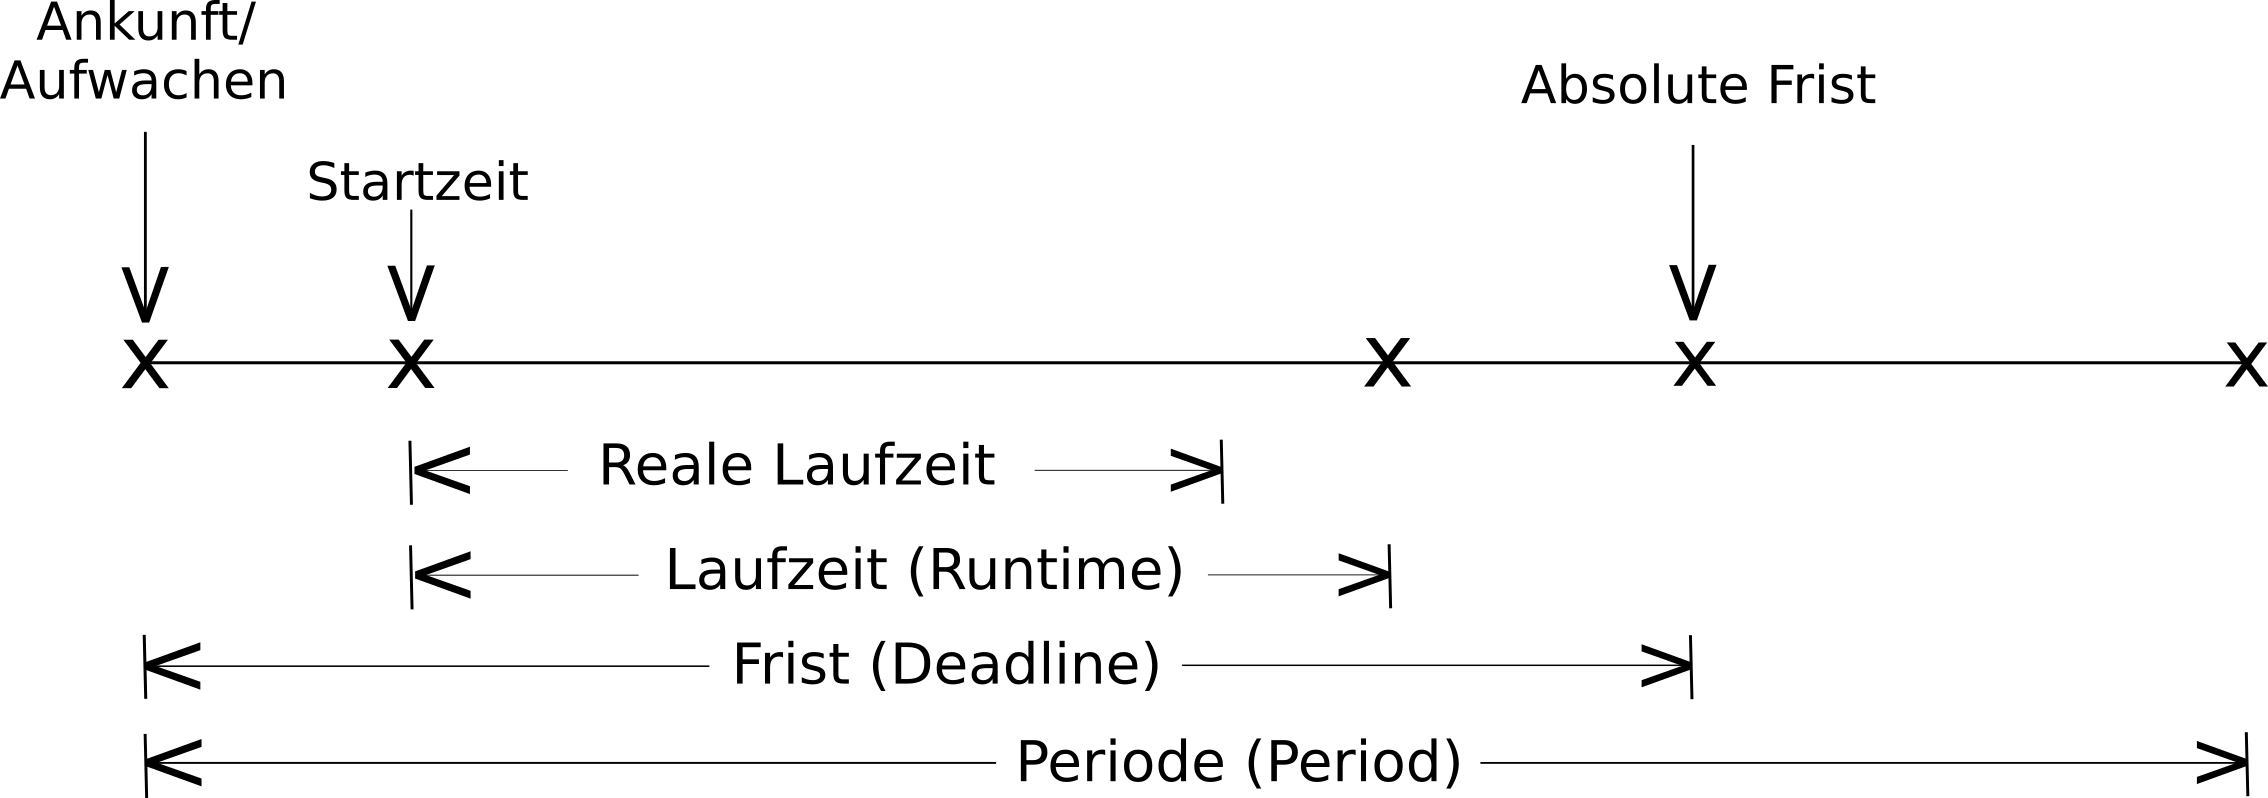
\includegraphics[width=0.85\textwidth]{images/anhang/sched_deadline}
	\caption[Ablauf von SCHED\_DEADLINE]{Ablauf von SCHED\_DEADLINE\\Quelle: Eigene Darstellung, in Anlehnung an \cite{man_sched7_nodate}}
	\label{fig:sched_deadline}
\end{figure}
\FloatBarrier

Für den \quoteMark{SCHED\_DEADLINE}-Scheduler müssen hierfür die Parameter, welche in Abbildung \ref{fig:sched_deadline} ersichtlich sind, richtig eingestellt werden. Der \quoteMark{Runtime}-Parameter beträgt zur Einhaltung der 50 ms Frist hierbei 50000000 ns, der \quoteMark{Deadline}-Parameter beträgt 50000000 ns und der \quoteMark{Periode}-Parameter beträgt 50000000 ns. Der \quoteMark{Runtime}-Parameter steht hierbei für die maximal benötigte Ausführungszeit der Aufgabe, der \quoteMark{Deadline}-Parameter für wie lange genügend Zeit vorhanden ist um die Aufgabe auszuführen und der \quoteMark{Periode}-Parameter für wann die nächste Periode gestartet werden muss \cite{man_sched7_nodate}. Diese Einstellungen wurden im Listing \ref{lst:settings_for_start_script} bei den Bash Variablen \quoteMark{SCHED\_RUNTIME}, \quoteMark{SCHED\_DEADLINE} und \quoteMark{SCHED\_PERIOD} im Start-Script bereits voreingestellt.\\

\begin{lstlisting}[style=bash, caption={Einstellungen des Start-Scripts der Roboter-Gesten-Anwendung}, label={lst:settings_for_start_script}]
USE_ROS_COMMUNICATION=true
USE_SIMULATION=true  # Only usable with "USE_ROS_COMMUNICATION=true"
DO_MEASUREMENT=false  # Only usable with "USE_SIMULATION=false" and
                       # "USE_ROS_COMMUNICATION=true"
SIMULATE_ADDITIONAL_ROS_NODES=false  # Only usable with "DO_MEASUREMENT=true"
ADDITIONAL_ROS_NODES_COUNT=3  # Only usable with "SIMULATE_OTHER_ROS_NODES=true"
LXC_USER_NAME="ubuntu"
LXC_INSTANCE="<container name>"
ADDITIONAL_APP_PARAMETERS="--move-home-at-exit --move-home-at-error"
TEACH_POSITIONS=true  # If "true" positions can be teached. Otherwise the positions
                        # in the file "robot_arm_positions.json" will be executed.
CONFIGURATION_FILE_PATH=""  # Empty for the default file path
                              # ("~/robot_arm_positions.json")
SCHED_RUNTIME=50000000
SCHED_DEADLINE=50000000
SCHED_PERIOD=50000000
\end{lstlisting}\leavevmode\newline\vspace{-1.0em}

Die Roboter-Gesten-Anwendung kann mit dem Start-Script \quoteMark{start\_tir.sh}, welches sich auf der CD/ISO im Verzeichnis \quoteMark{Repositories/Teach-Industrial-Robots} befindet, auf dem Host-System im Linux-Container gestartet und dem \quoteMark{SCHED\_DEADLINE}-Scheduler zugewiesen werden. Die einstellbaren Optionen des Start-Scripts sind im Listing \ref{lst:settings_for_start_script} ersichtlich. Zum Ausführen des Start-Scripts muss im Listing \ref{lst:settings_for_start_script} die Bash-Variable \quoteMark{LXC\_INSTANCE} mit dem Namen des Linux-Containers ersetzt werden. Die Bash-Variable \quoteMark{USE\_ROS\_COMMUNICA-\\TION} steuert ob die Roboter-Gesten-Anwendung über ROS kommunizieren oder eine direkt Verbindung mit dem Industrieroboter aufbauen soll. Um der Roboter-Gesten-Anwendung mitteilen zu können ob diese im Lern- oder Abspielmodus gestartet werden soll, wird die Bash-Variable \quoteMark{TEACH\_POSITIONS} eingesetzt. Zur Auswahl der verwendeten Positionsdatei kann die Bash-Variable \quoteMark{CONFIGURATION\_FILE\_PATH} mit dem Pfad zur Positionsdatei genutzt werden. Mit der Bash-Variable \quoteMark{USE\_SIMULATION} kann eingestellt werden ob die Anwendung im Simulator gestartet werden soll. Die Bash-Variable \quoteMark{DO\_MEASUREMENT} kann bei Verwendung eines echten Industrieroboters dazu verwendet werden um Messvorraussetzungen, wie z.B. ein simuliertes Netzwerk, bereitzustellen. Zudem kann bei aktivierter \quoteMark{DO\_MEASUREMENT}-Bash-Variable die Bash-Variable \quoteMark{SIMULATE\_ADDITIONAL\_ROS\\\_NODES} aktiviert werden um zusätzlichen Netzwerktraffik zu generieren. Mit der Bash-Variable \quoteMark{ADDITIONAL\_ROS\_NODES\_COUNT} kann bei aktivierter \quoteMark{SIMULATE\_ADD-\\ITIONAL\_ROS\_NODES}-Bash-Variable auch die Anzahl der zu simulierenden ROS-Nodes angegeben werden. Es werden Kamera-ROS-Nodes simuliert, welche jeweils 4K-Bilder mit 60 FPS per UDP über die Netzwerkschnittstelle transferieren. Um weitere von der Roboter-Gesten-Anwendung unterstützte Parameter anwenden zu können, kann die Bash-Variable \quoteMark{ADDITIONAL\_APP\_PARAMETERS} mit den nachstehenden Parametern modifiziert werden.

\begin{longtable}{|>{\raggedright\arraybackslash}p{0.2\textwidth}|>{\raggedright\arraybackslash}p{0.20\textwidth}|>{\raggedright\arraybackslash}p{0.50\textwidth}|}
\hline
\rowcolor{LightGray} \thead[c]{Kurzschreibweise\\des\\Parameters} & \thead[c]{Ausgeschriebener\\Parameter} & \thead[c]{Beschreibung}\\
\hline
-pfp="\phantom{}<path>" & \texttt{-{}-}positions-file-path="\phantom{}<path>" & Dateipfad zum Speichern oder Laden der aufgezeichneten Positionen \newline (Default-Positionsdateipfad: "\~{}/robot\_arm\_positions.json")\\
\hline
-opf & \texttt{-{}-}overwrite-positions-file & Ermöglicht das Überschreiben der Positionsdatei. Zuvor sollte ein Backup der Positionsdatei gemacht werde um Datenverlust zu vermeiden.\\
\hline
-rrp & \texttt{-{}-}repeat-recorded-positions & Die aufgezeichneten Positionen aus der Positionsdatei wiederholen lassen\\
\hline
-tp & \texttt{-{}-}teach-positions & Positionen lernen\\
\hline
-rn="\phantom{}<name>" & \texttt{-{}-}robot-name="\phantom{}<name>" & Name des Roboters\newline (Default: "wx200")\\
\hline
-rm="\phantom{}<model>" & \texttt{-{}-}robot-model="\phantom{}<model>" & Robotermodell\newline (in der Regel der Name des Roboters\newline Default: "wx200")\\
\hline
-ur & \texttt{-{}-}use-ros & ROS oder eine direkte Verbindung zum Industrieroboter verwenden\\
\hline
-mhaex & \texttt{-{}-}move-home-at-exit & Beim Beenden der Anwendung in die Ausgangsposition zurückfahren\\
\hline
-mhaer & \texttt{-{}-}move-home-at-error & Bei einem Fehler der Anwendung in die Ausgangsposition zurückfahren\\
\hline
 & --help & Zeigt die Hilfe\\
\hline
\end{longtable}

%-----------------------------------------------

% Scheduler wechseln:
% cat /sys/block/sda/queue/scheduler

%-------------

% https://www.researchgate.net/publication/331290349_The_real-time_linux_kernel_A_survey_on_Preempt_RT

% -----------

% verwendeter Tiefensensor-Modus -> warum?

% Intel Real Sense Camera ZR300

%-------------------


% https://books.google.at/books?id=vVMoDwAAQBAJ&pg=PA229&lpg=PA229&dq=lxc+realtime&source=bl&ots=6aSRy33GKg&sig=ACfU3U13TeQVx0D1fZ5Z6DxLmKdeHTkXOg&hl=de&sa=X&ved=2ahUKEwj3mrWgyuvpAhUEGuwKHdcmDr8Q6AEwA3oECAoQAQ#v=onepage&q=lxc%20realtime&f=false


% Literaturverzeichnis:
\clearpage
\phantomsection
\addcontentsline{toc}{chapter}{Literaturverzeichnis}
\printbibliography


\chapter*{Eidesstattliche Erklärung}
\addcontentsline{toc}{chapter}{Eidesstattliche Erklärung}
Ich erkläre hiermit an Eides statt, dass ich die vorliegende Masterarbeit selbstständig und ohne Benutzung anderer als der angegebenen Hilfsmittel angefertigt habe. Die aus fremden Quellen direkt oder indirekt übernommenen Stellen sind als solche kenntlich gemacht. Die Arbeit wurde bisher weder in gleicher noch in ähnlicher Form einer anderen Prüfungsbehörde vorgelegt und auch noch nicht veröffentlicht.

\vspace{3cm}
\noindent
Dornbirn, am \today %[Tag. Monat Jahr anführen]
\hfill Helmut Rhomberg %[Vor- und Nachname Verfasser/in]


\end{document}
